\section{Vortex formation at planetary gap edges in layered
  discs}\label{disc-planet} 
The previous simulations, while necessary to isolate the effect of 
viscosity on the linear RWI, has the disadvantage that the radially
structured viscosity profile can act to source radial disc structure
in the non-linear regime. In this section, we employ a radially smooth
viscosity profile and use 
disc-planet interaction to
create the disc structure required for instability. We therefore expect viscosity to only
act as a damping mechanism. 

Vortex formation at gap edges is a standard result in 
2D and 3D hydrodynamical simulations of giant planets in low viscosity discs 
\citep{valborro07,lin10,lin11a,lin12}. The fact that this is due to
the RWI has been explicitly verified through linear stability
analysis %of planetary gap profiles produced from 2D simulations
\citep{valborro07,lin10}. Here, we simulate gap-opening giant planets
in 3D discs where the kinematic viscosity varies with height above the
disc midplane. Our numerical experiments are similar in spirit to
those performed by \cite{pierens10}, but our focus here is gap
stability in a layered disc. 
 
\subsection{Radially smooth viscosity profile for disc-planet
  interaction}\label{planet_visc_mode} 
Using the same notation as \S\ref{visc_model}, we impose a viscosity
profile $\hat{\nu}$ such that 
\begin{align}\label{planet_visc_profile}
  \hat{\nu}\Sigma_i(R)=
  \hat{\nu}_0\left[1+Q(\psi)\right]\Sigma_i(r_0)   
\end{align}
We have set the dimensionless argument in Eq. \ref{step} to
$\zeta=\psi$. Recall $\psi=\pi/2-\theta$ is the angular height away from the midplane. 
The viscosity increases from its floor value $\hat{\nu}_0$ by a factor
$A_\nu$ for $\psi > \zeta_\nu$. So the viscous layer is 
a wedge in the meridional plane, which conveniently fits into our
spherical grid. %The floor viscosity is $\hat{\nu}_0=2.5\times 10^{-7}$
%or $\hat{\nu}_0=10^{-6}$. 
The angular thickness of the viscosity
transition is fixed to $\Delta\zeta_\nu =
0.2h$. Fig. \ref{planet_visc2d} gives an example of this  
viscosity profile. 

\begin{figure}
  \centering
  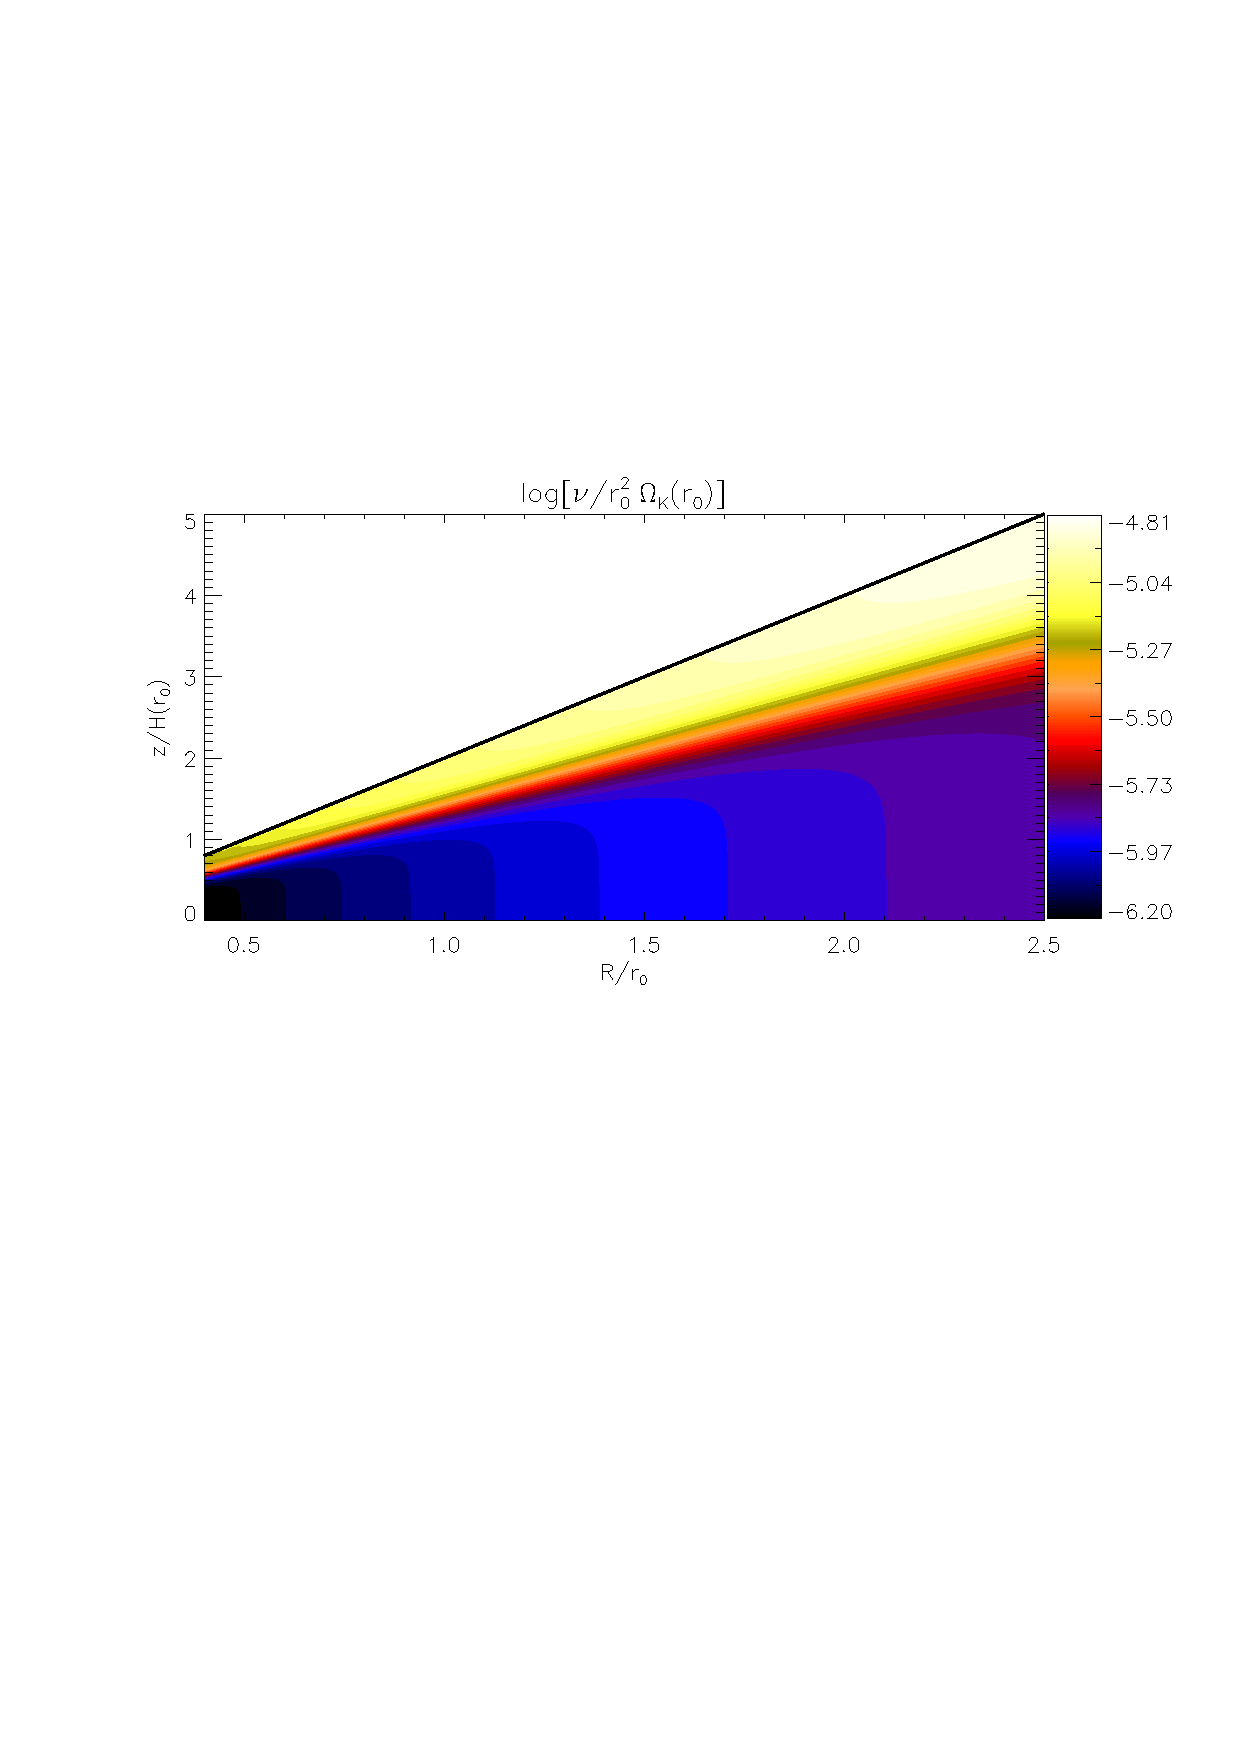
\includegraphics[width=\linewidth]{figures/pdisk_visc2d_planet}
  \caption{Example of the viscosity profile
    imposed in disc-planet simulations
    (Eq. \ref{planet_visc_profile}).  
    For a disc with constant aspect ratio, the viscous
    layer occupies a constant number of scale heights across the
    radial range. This specific plot corresponds to case P1, so the
    viscous layer (yellow-white colours) always occupies the uppermost
    $H$ at each cylindrical radius. 
    The solid line delineates the upper boundary of the computational
    domain. 
    \label{planet_visc2d}}
\end{figure}

\subsection{Disc-planet simulations} 
We simulate locally isothermal discs with constant aspect-ratio
$h=0.05$ (by choosing $q=1$), vertical extent $n_h=3$ scale-heights 
and radial extent $[\rin,\rout]=[0.4,2.5]r_0$. Initially the surface density is smooth
($A=1$) with zero meridional velocity ($v_r=v_\theta=0$). 
%cylindrical radial velocity is given by
%Eq. \ref{init_vr}. 
The standard resolution is $(N_r, N_\theta,
N_\phi)=(256, 96, 768)$, corresponding to $6,\,32,\,6$ 
cells per $H$ along the $r,\theta,\phi$ directions at the reference
radius. We apply a damping rate $\hat{\gamma}=2$ with the reference
velocity field $\bm{v}_\mathrm{ref}=(0,0,v_\phi)$ in spherical
co-ordinates.   

We insert into the disc a planet of mass  
$M_p=10^{-3}M_*$, which corresponds to a Jupiter mass planet if
$M_*=M_{\sun}$. The softening length for the planet potential is
$\epsilon_p=0.5r_h$. The planet potential is switched on 
smoothly over $t\in[0,10]P_0$. We note that the disc can be considered
as two-dimensional for gap-opening giant planets, because the Hill
radius $r_h$ exceeds the local scale-height $H$ ($r_h/H\simeq1.4$
in our cases).   

We remark that, apart from the viscosity prescription, the above
choice of physical and numerical parameter values are typical for
global disc-planet simulations \citep[e.g.][]{valborro06,mignone12}.    


%%%%%%%%%%%%%%%%%%%%%%%%%%%%%%%%%%%%%%%%%%%%%%%%%%%%%%%%%%%%%%%%%%%%%%%%%%%%%%%


\subsection{Results}
Table \ref{planet_sims} summarizes the disc-planet simulations. 
%\subsubsection{Runs} 
The main simulations to be discussed are cases P0 --- P1, with a floor
viscosity of $\hat{\nu}_0=2.5\times10^{-7}$. 
The fiducial run P0 has $A_\nu=1$, i.e. no viscous layer, so 
$\hat{\nu}\sim 10^{-7}$ ($\alpha\sim 10^{-4}$) everywhere. 
The typical viscosity value adopted for disc-planet simulations,
$\hat{\nu}\sim 10^{-5}$ or $\alpha\sim 10^{-3}$, is known to suppress vortex formation
\citep{valborro07, mudryk09}. Thus vortex formation is expected for
case P0. For case P0.5 and P1 we set $A_\nu=100$ with transition angle $\zeta_\nu=2.5h$ and
$2h$, respectively, so the viscous layer with $\hat{\nu}\sim10^{-5}$
($\alpha\sim10^{-2}$) occupies the uppermost $0.5H$ and $H$ of the vertical
domain. Case P0R is case P0 restarted from 
$t=100P_0$ with the layered viscosity profile of case P1. 
 

\begin{table*}
  \centering
  \caption{Summary of disc-planet simulations. These runs employ the
    `wedge' viscosity model described by
    Eq. \ref{planet_visc_profile}. The thickness of the viscous layer
    is measured from the upper disc boundary. The $m=1$ mode amplitude was 
    averaged over the shell $r\in[1.2,1.6]r_0$; and the overbar
    denotes a further time average over    
    $t\in[t_\mathrm{max},200]P_0$, where $t_\mathrm{max}$ is when
    $\mathrm{max}(a_1)$ is attained. Case P0R employs the
    viscosity profile of P0 for $t\leq100P_0$, and that of P1 for 
    $t>100P_0$.\label{planet_sims}}
    \begin{tabular}{llllrrl}
      \hline\hline
      Case & $10^6\hat{\nu}_0$ & $A_\nu$ & visc. layer&
      $10^2\overline{a}_1$&$10^2a_1(200P_0)$ & comment \\ 
      \hline
      P0     & 0.25  & 1            & 0     & 18.3  & 14.5 & single vortex
       by $t=130P_0$ and persists until end of sim.  \\ %doing HR
      P0.5   & 0.25  & 100          & $0.5H$ &  17.4  & 8.6& single vortex
      by $t=90P_0$ and persists until end of sim.\\ 
      P0R    & 0.25  & 1$\to$100    & $0\to H$& 10.1 & 2.5& single vortex
      by $t=130P_0$, disappears after $t=180P_0$ \\
      P1     & 0.25  & 100          & $H$    & 12.5  & 2.1 &single vortex
      by $t=80P_0$, disappears after $t=170P_0$ \\   %doing HR
      

      Pb0     & 1.0  & 1          & 0      & 9.2  & 5.4 &single vortex by $t=130P_0$, disappears
      vortex after $t=160P_0$   \\ %doing HR
      Pb0.5   & 1.0  & 10         & $0.5H$ & 7.3  & 3.0 &similar to Pb0     \\ 
      Pb1     & 1.0  & 10         & $H$    & 5.7  & 2.2   &single vortex
      by $t=120P_0$, disappears after $t=140P_0$   \\ %doing HR

      Pc0.5   & 1.0  & 100          & $0.5H$ & 4.2  &  2.3 &two vortices
      at $t\sim100P_0$, no vortices after $t\sim120P_0$   \\ %optional
      Pc1     & 1.0  & 100          & $H$    & 2.2 &  1.6 &two weak vortices at
      $t\sim60P_0$, no vortices after $t\sim 80P_0$\\ %optional  
      \hline
  \end{tabular}
\end{table*}

%other sims
%loc iso (q=1) with floor visc 1d-6, amp=100 and 10. HR for one of
%them. and visc-restart.  
%isothermal (q=0) with floor visc=1d-6, amp=100 and 10
%may need to add other columns nu_floor, nu_amp, q 

\subsubsection{Density evolution}%prob replace with nu_floor=1d-6,
                                %amp=10 sims

Fig. \ref{jup0_3h} compares the time evolution of the midplane density
perturbation $\delta\rho(z=0)$ for cases P0, P0.5 and P1. In 
all cases we observed the RWI with $m=4$ develops early on ($t\simeq20P_0$),
consistent with the limited effect of viscosity on the linear
instability, as found above.  

Comparing the no-layer case P0 to case P0.5 (viscous layer $0.5H$)
shows that a thin viscous layer has little effect on the
evolution of the unstable gap edge, except the vortex merging
time-scale is slightly altered. However, case P1 evolves quite
differently from case P0. While a single vortex does form at
$t\sim100P_0$ in case P1, it is \emph{transient}, having disappeared at the end of
the simulation. The final $m=1$ amplitude is about 3 times smaller
than that in case P0 (Table \ref{planet_sims}). This result is
significant because an upper viscous layer of 
thickness $H$ only occupies $\sim4\%$ of the total column density
in case P1, but the vortex is still destroyed. This suggests that vortex
survival at planetary gap edges requires low effective viscosity
throughout the vertical fluid column. 

\begin{figure*}
  \centering
  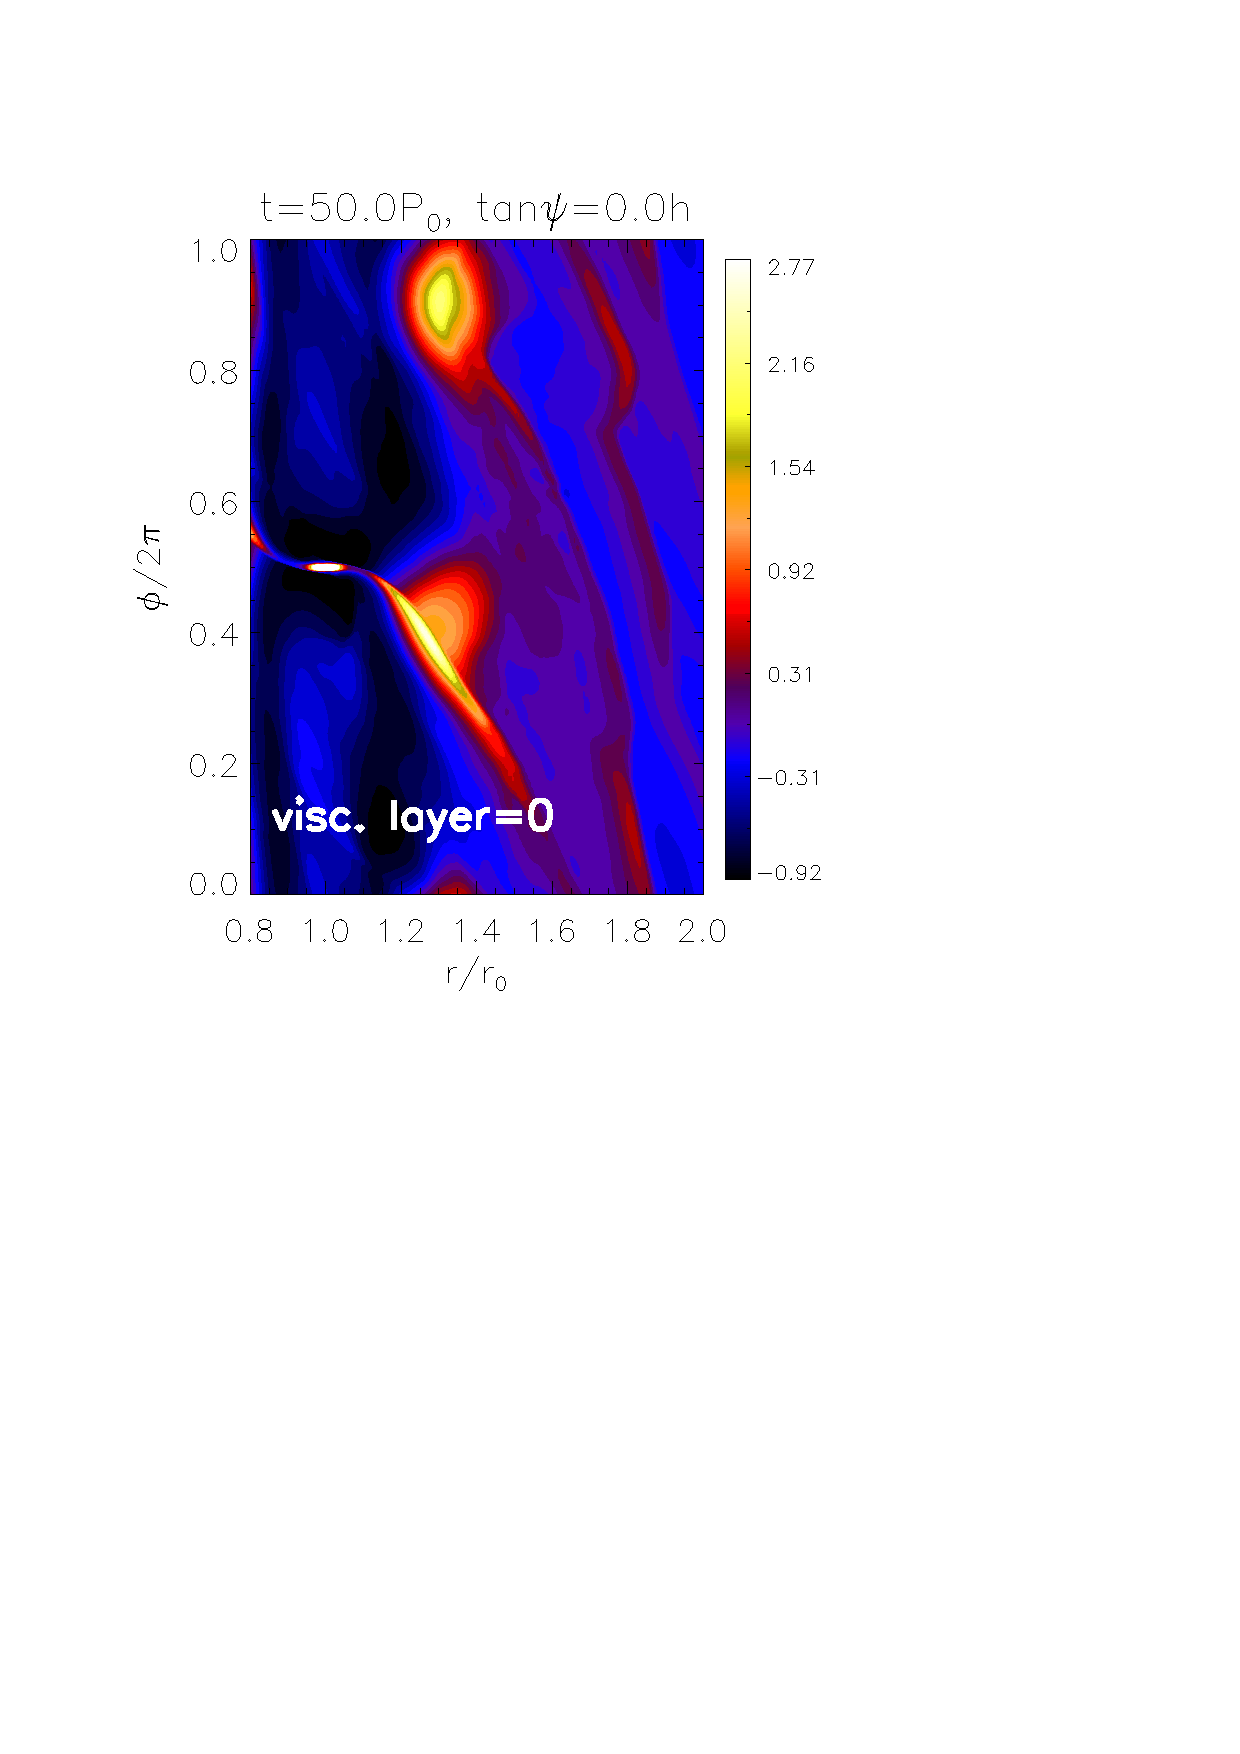
\includegraphics[scale=.43,clip=true,trim=0cm 1.84cm 0cm
    0cm]{figures/jup0_3h_pdisk_005}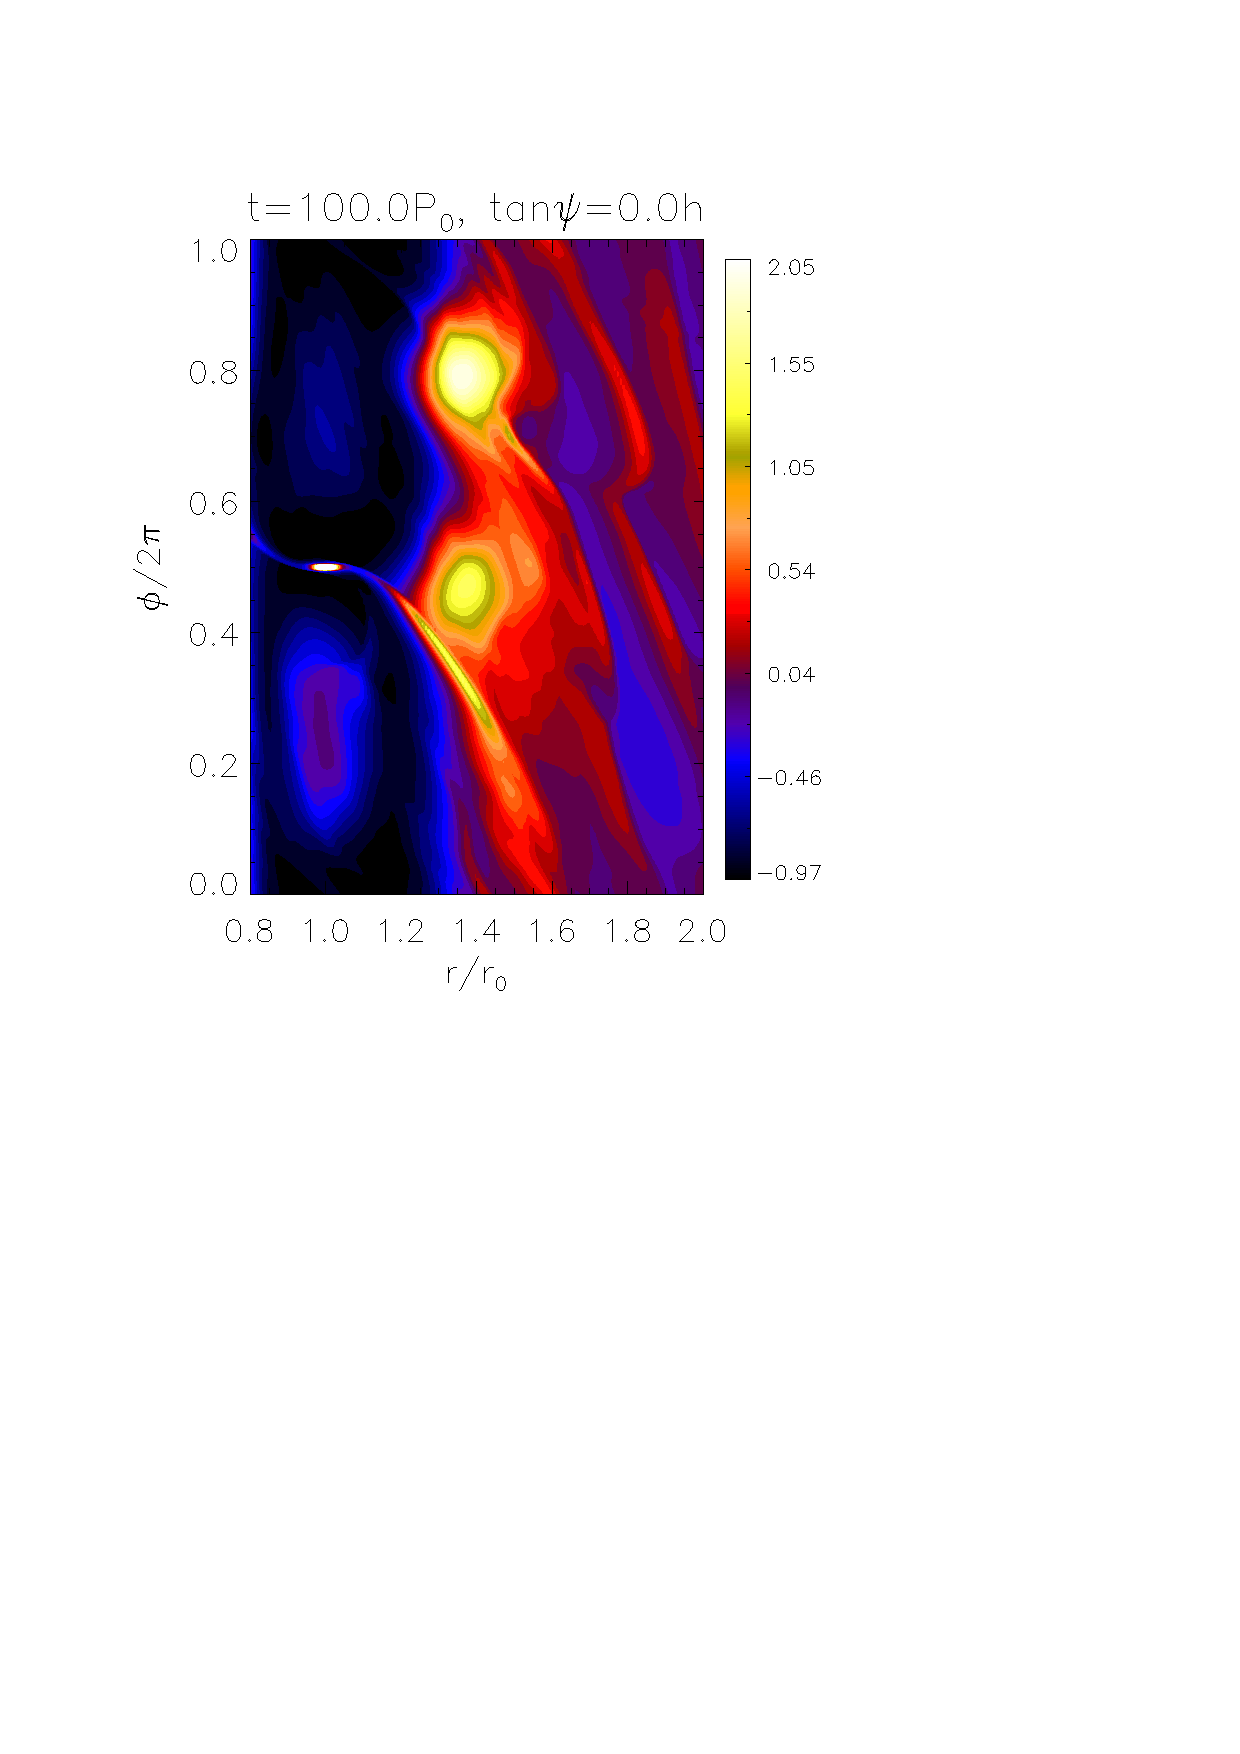
\includegraphics[scale=.43,clip=true,trim=2.3cm
    1.84cm 0cm 0cm]{figures/jup0_3h_pdisk_010}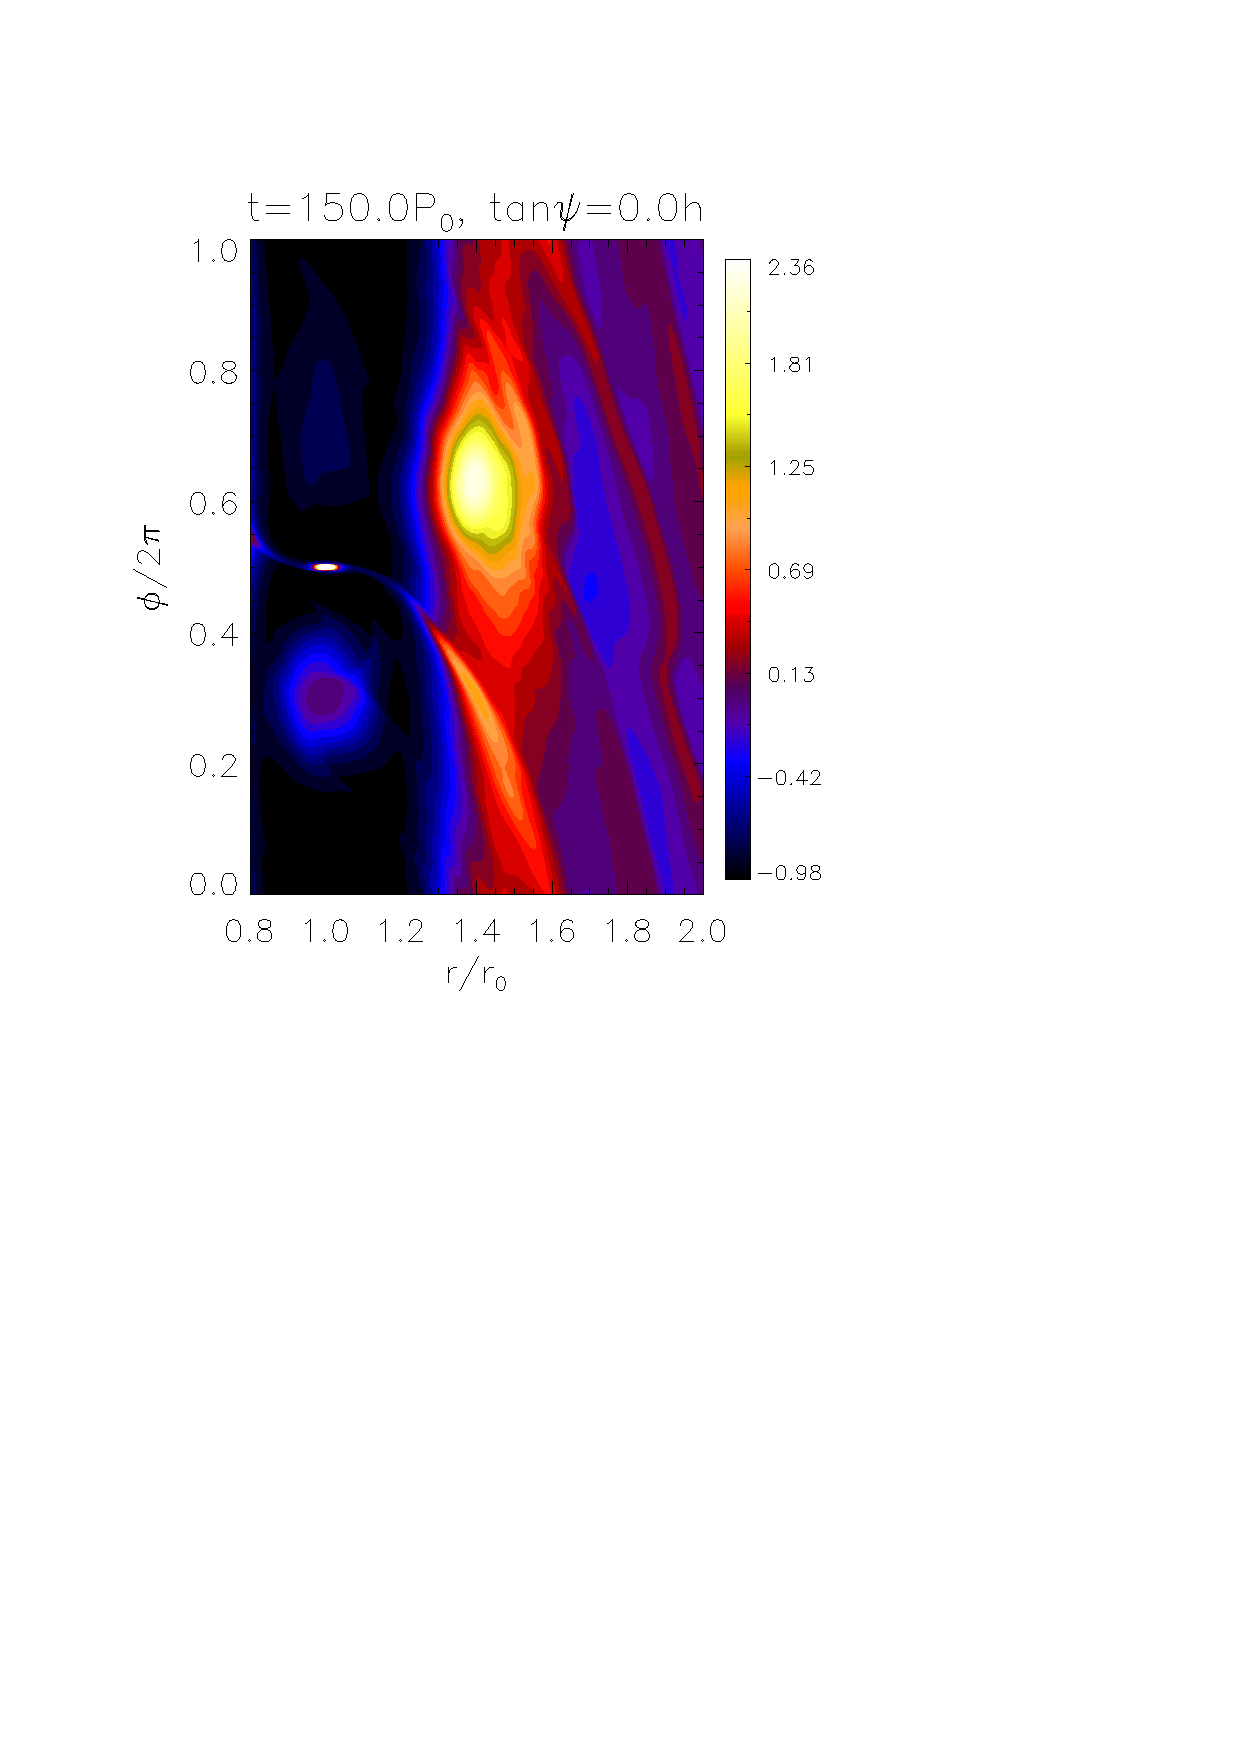
\includegraphics[scale=.43,clip=true,trim=2.3cm
    1.84cm 0cm 0cm]{figures/jup0_3h_pdisk_015}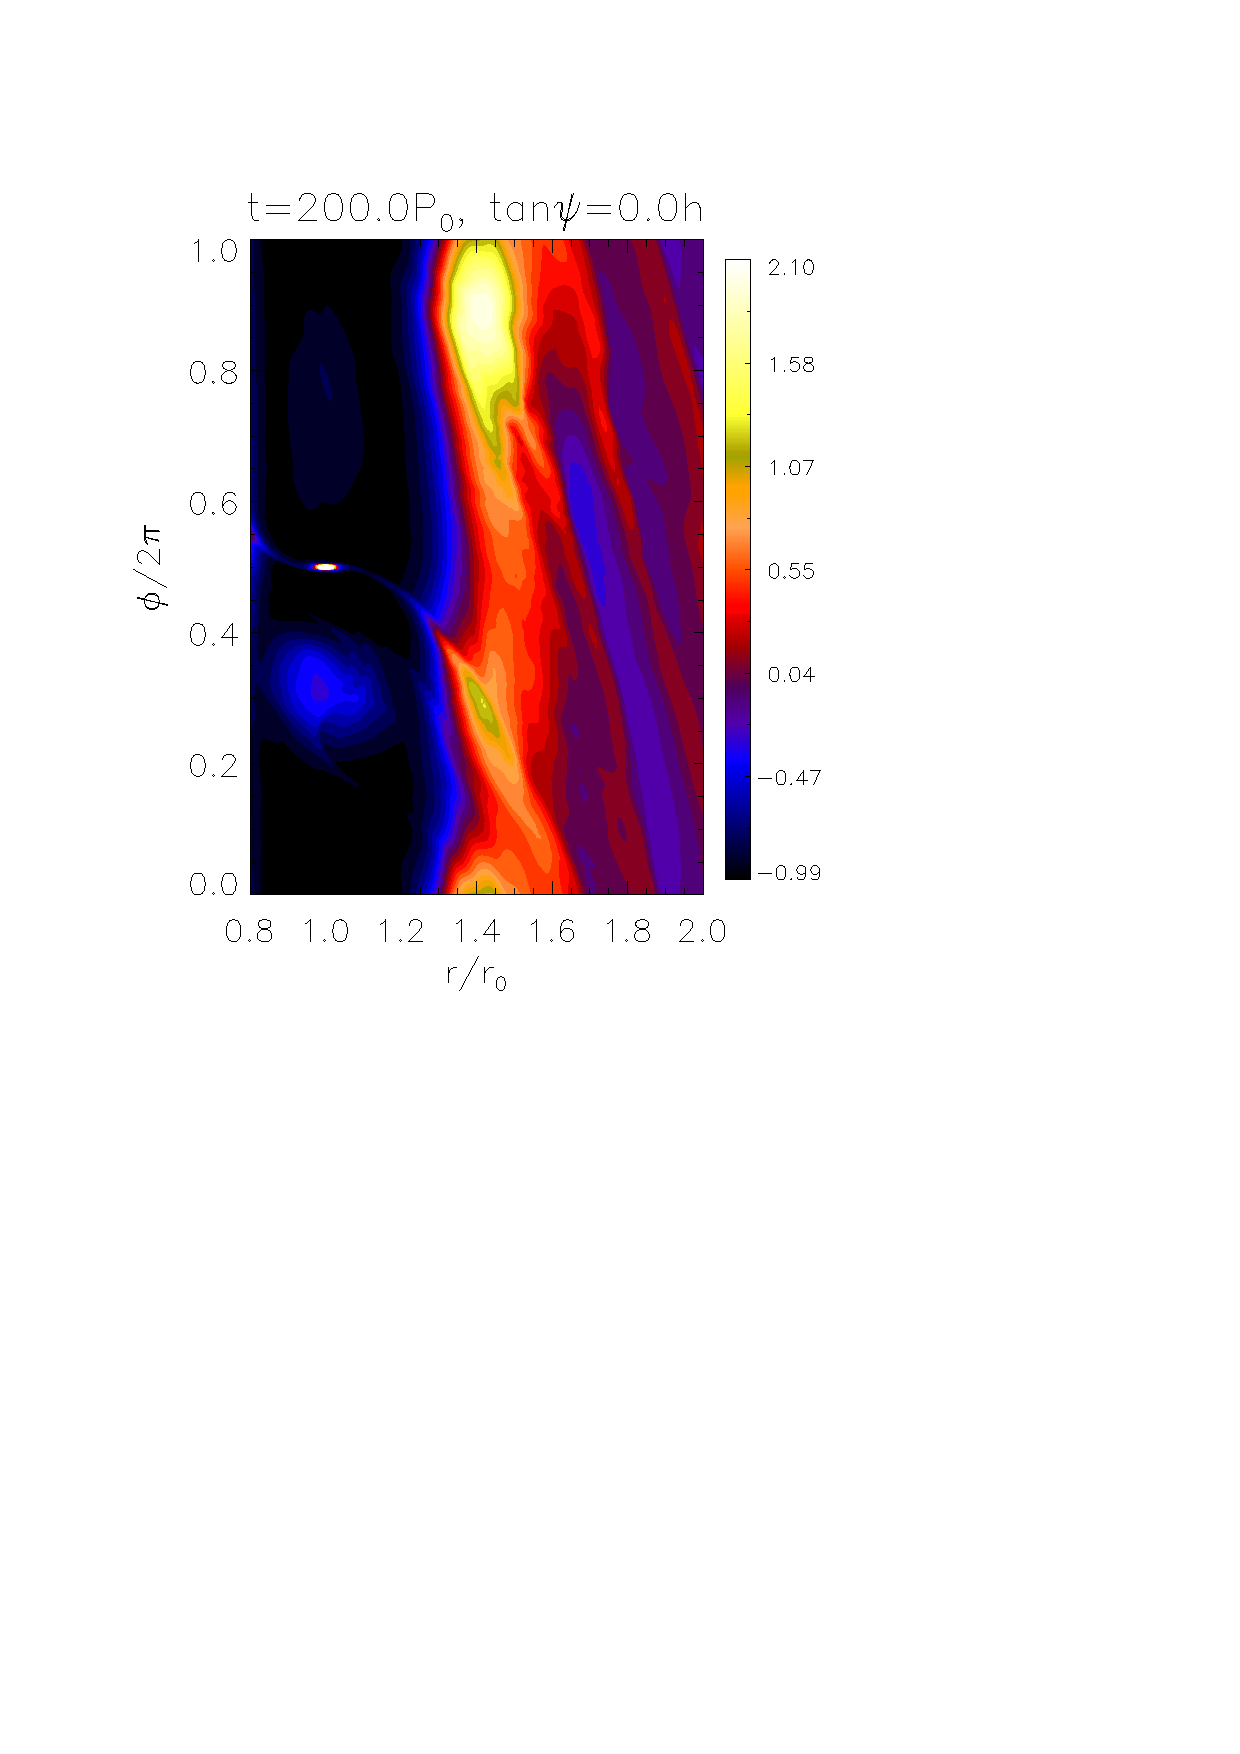
\includegraphics[scale=.43,clip=true,trim=2.3cm
    1.84cm 0cm 0cm]{figures/jup0_3h_pdisk_020}\\
%  \includegraphics[scale=.43,clip=true,trim=0cm 1.84cm 0cm
%    0.9cm]{figures/jup0d5_3h_pdisk_005.ps}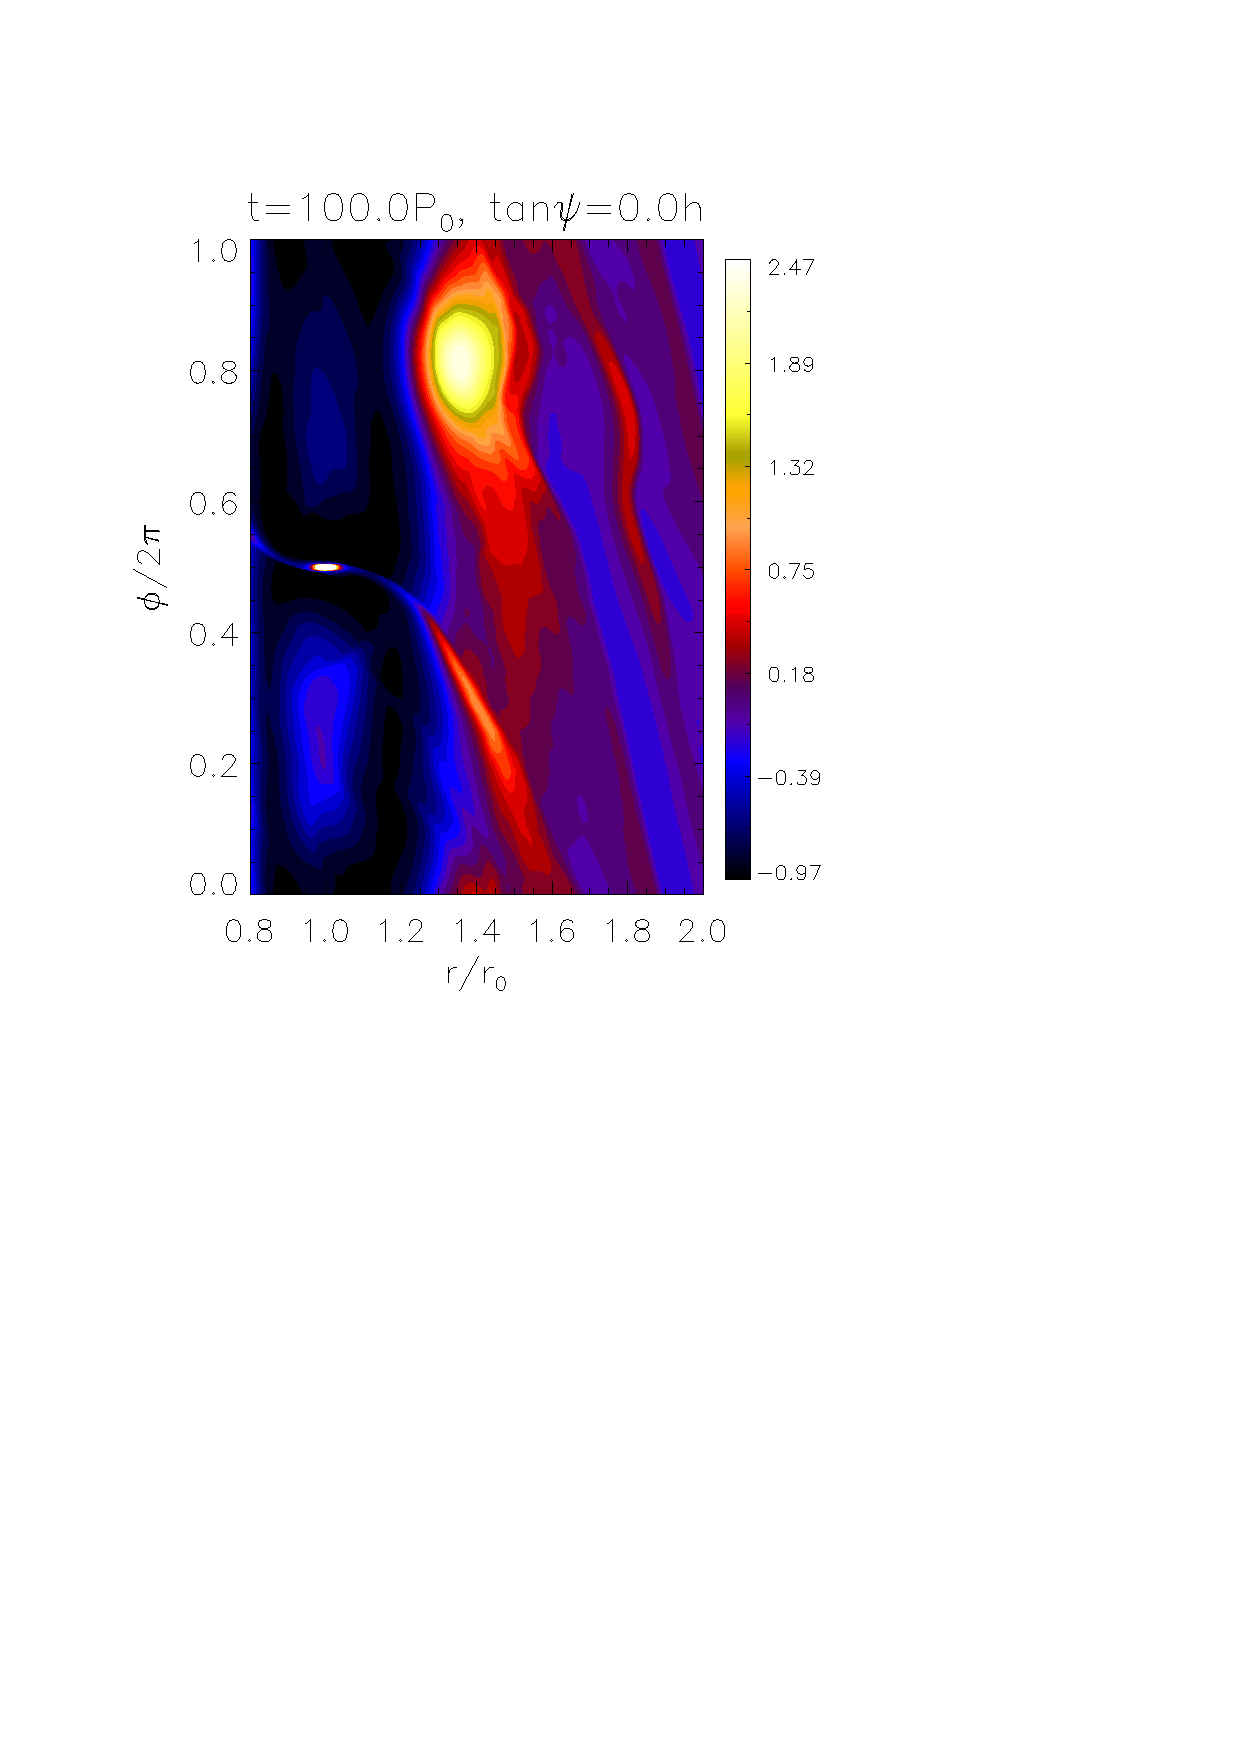
\includegraphics[scale=.43,clip=true,trim=2.3cm
%    1.84cm 0cm 0.9cm]{figures/jup0d5_3h_pdisk_010}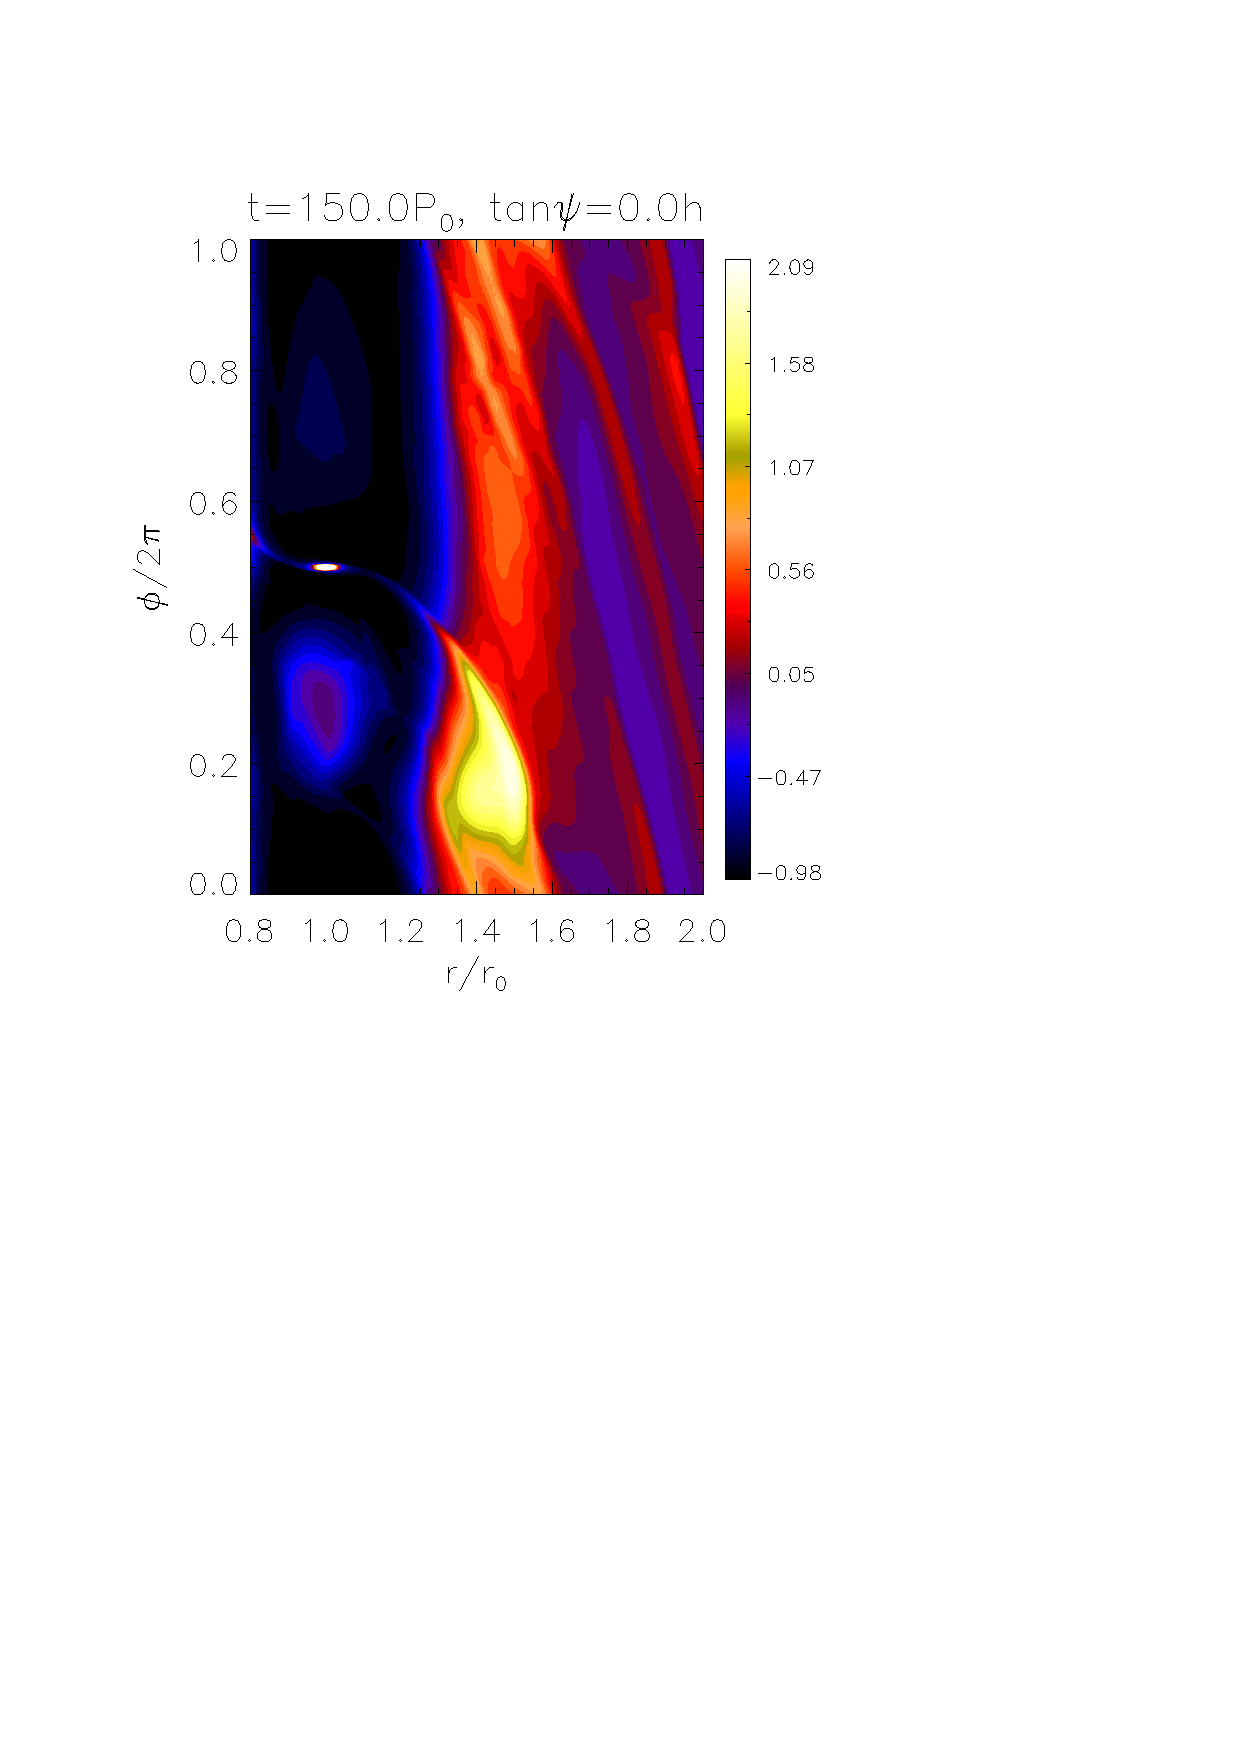
\includegraphics[scale=.43,clip=true,trim=2.3cm
%    1.84cm 0cm 0.9cm]{figures/jup0d5_3h_pdisk_015}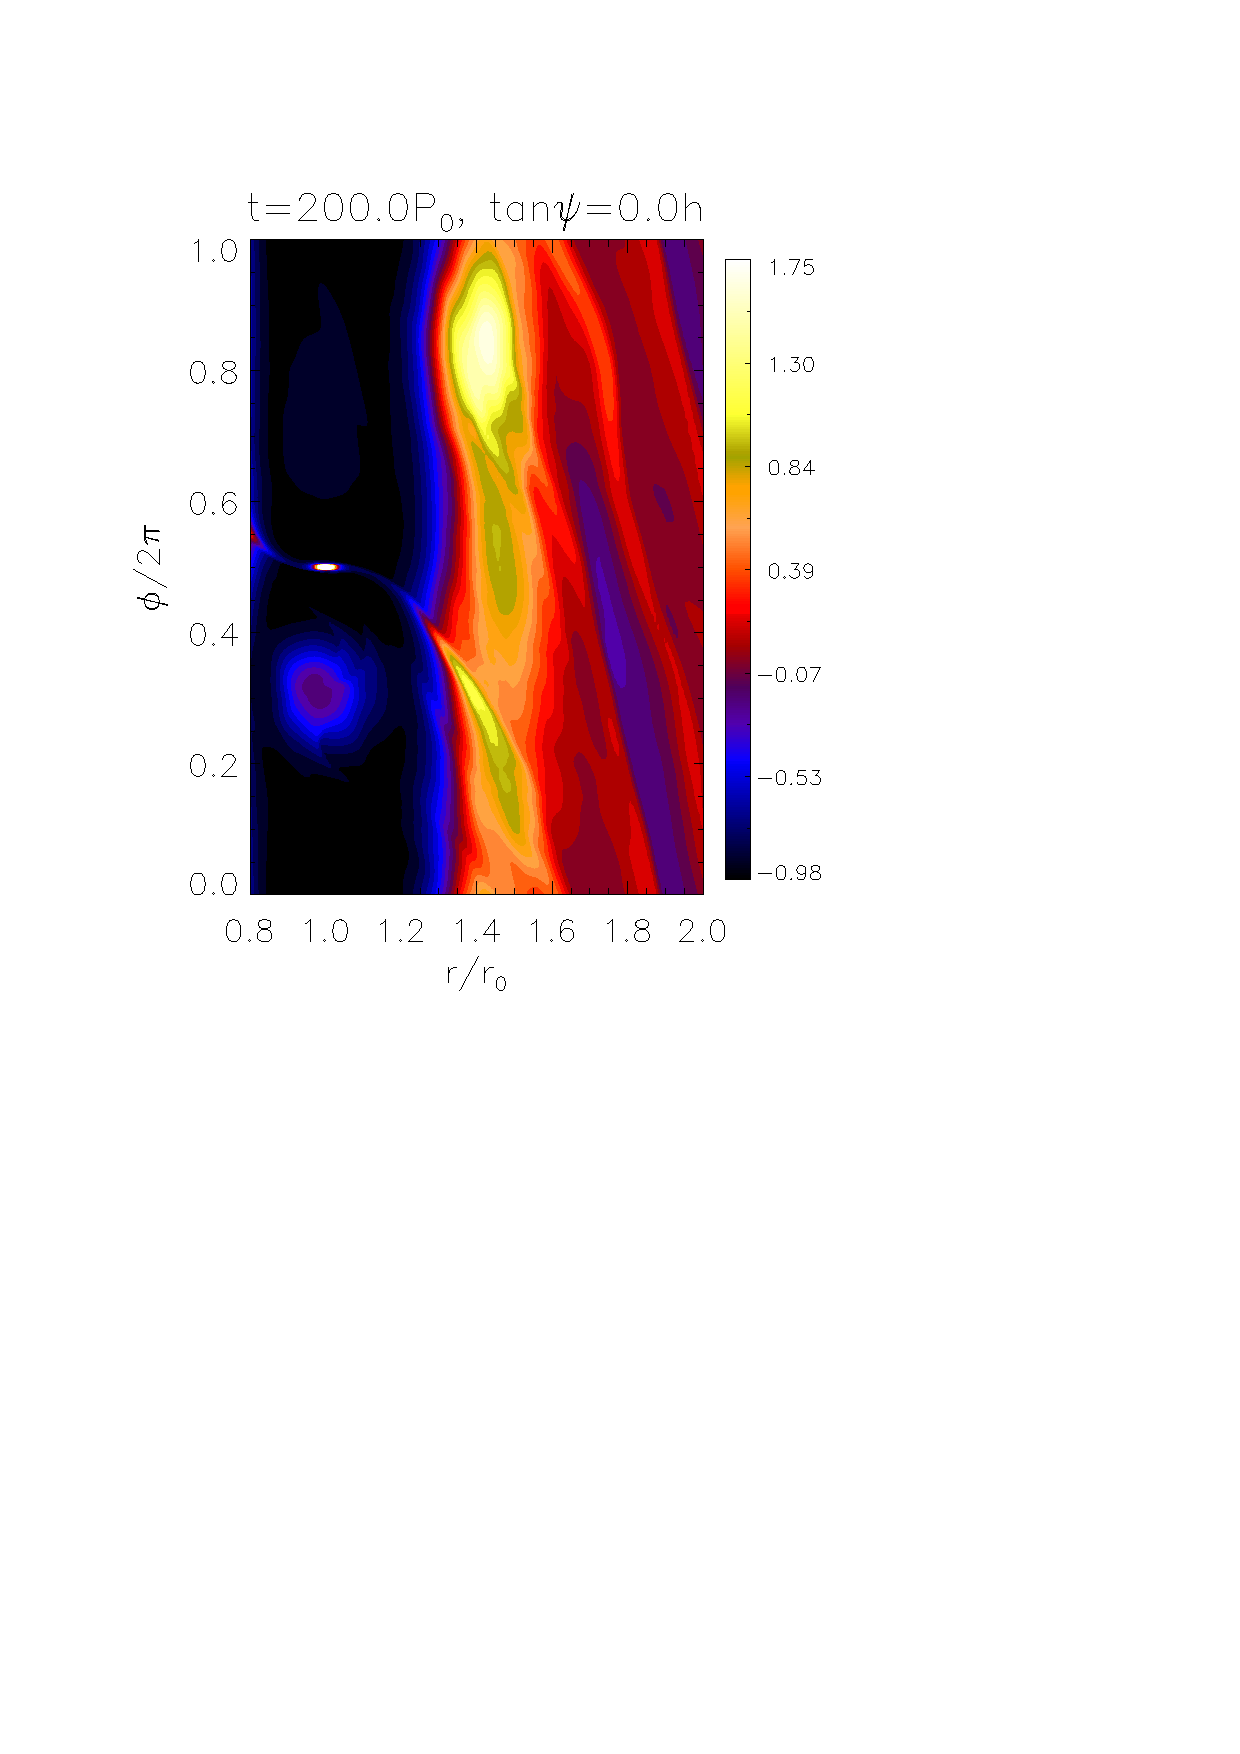
\includegraphics[scale=.43,clip=true,trim=2.3cm
%    1.84cm 0cm 0.9cm]{figures/jup0d5_3h_pdisk_020}\\
  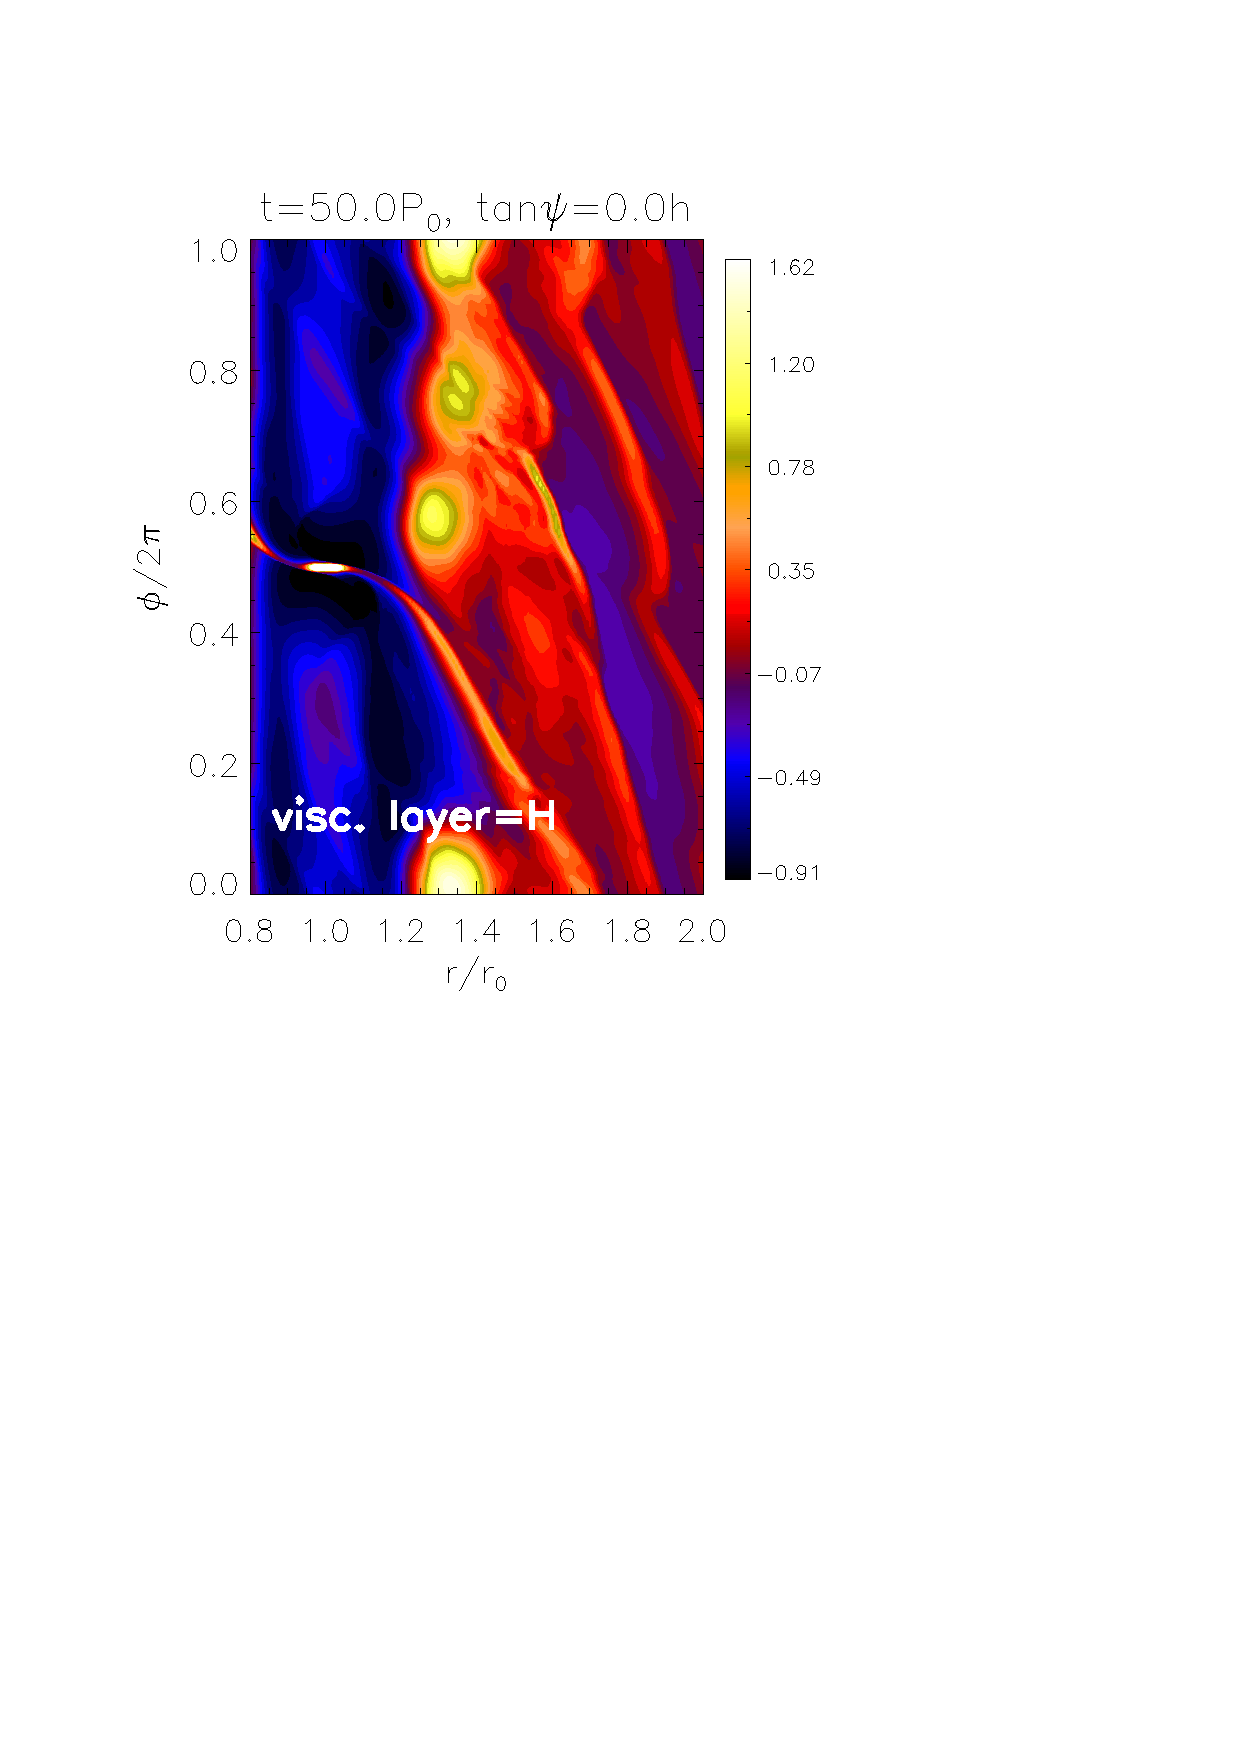
\includegraphics[scale=.43,clip=true,trim=0cm 0.cm 0.cm
    0.9cm]{figures/jup1_3h_pdisk_005}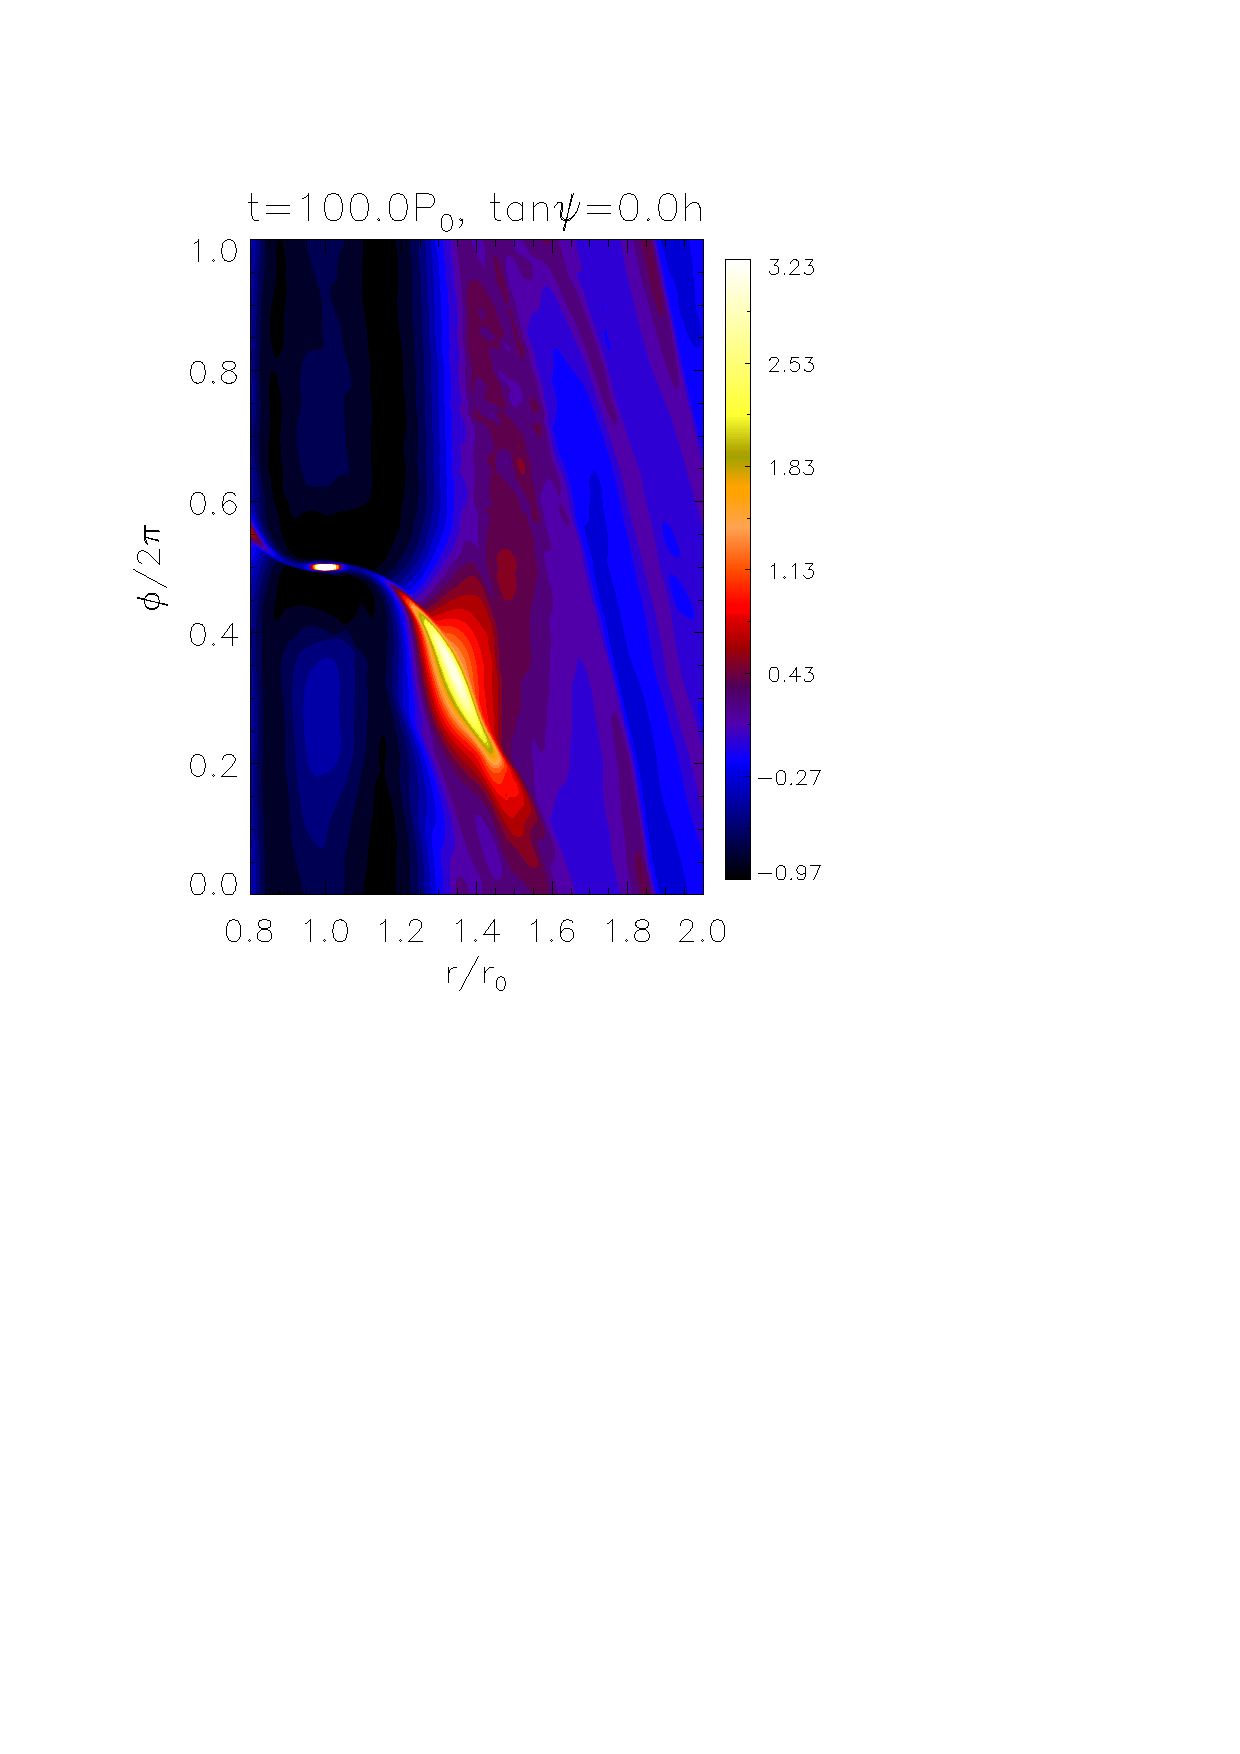
\includegraphics[scale=.43,clip=true,trim=2.3cm
    0.cm 0cm 0.9cm]{figures/jup1_3h_pdisk_010}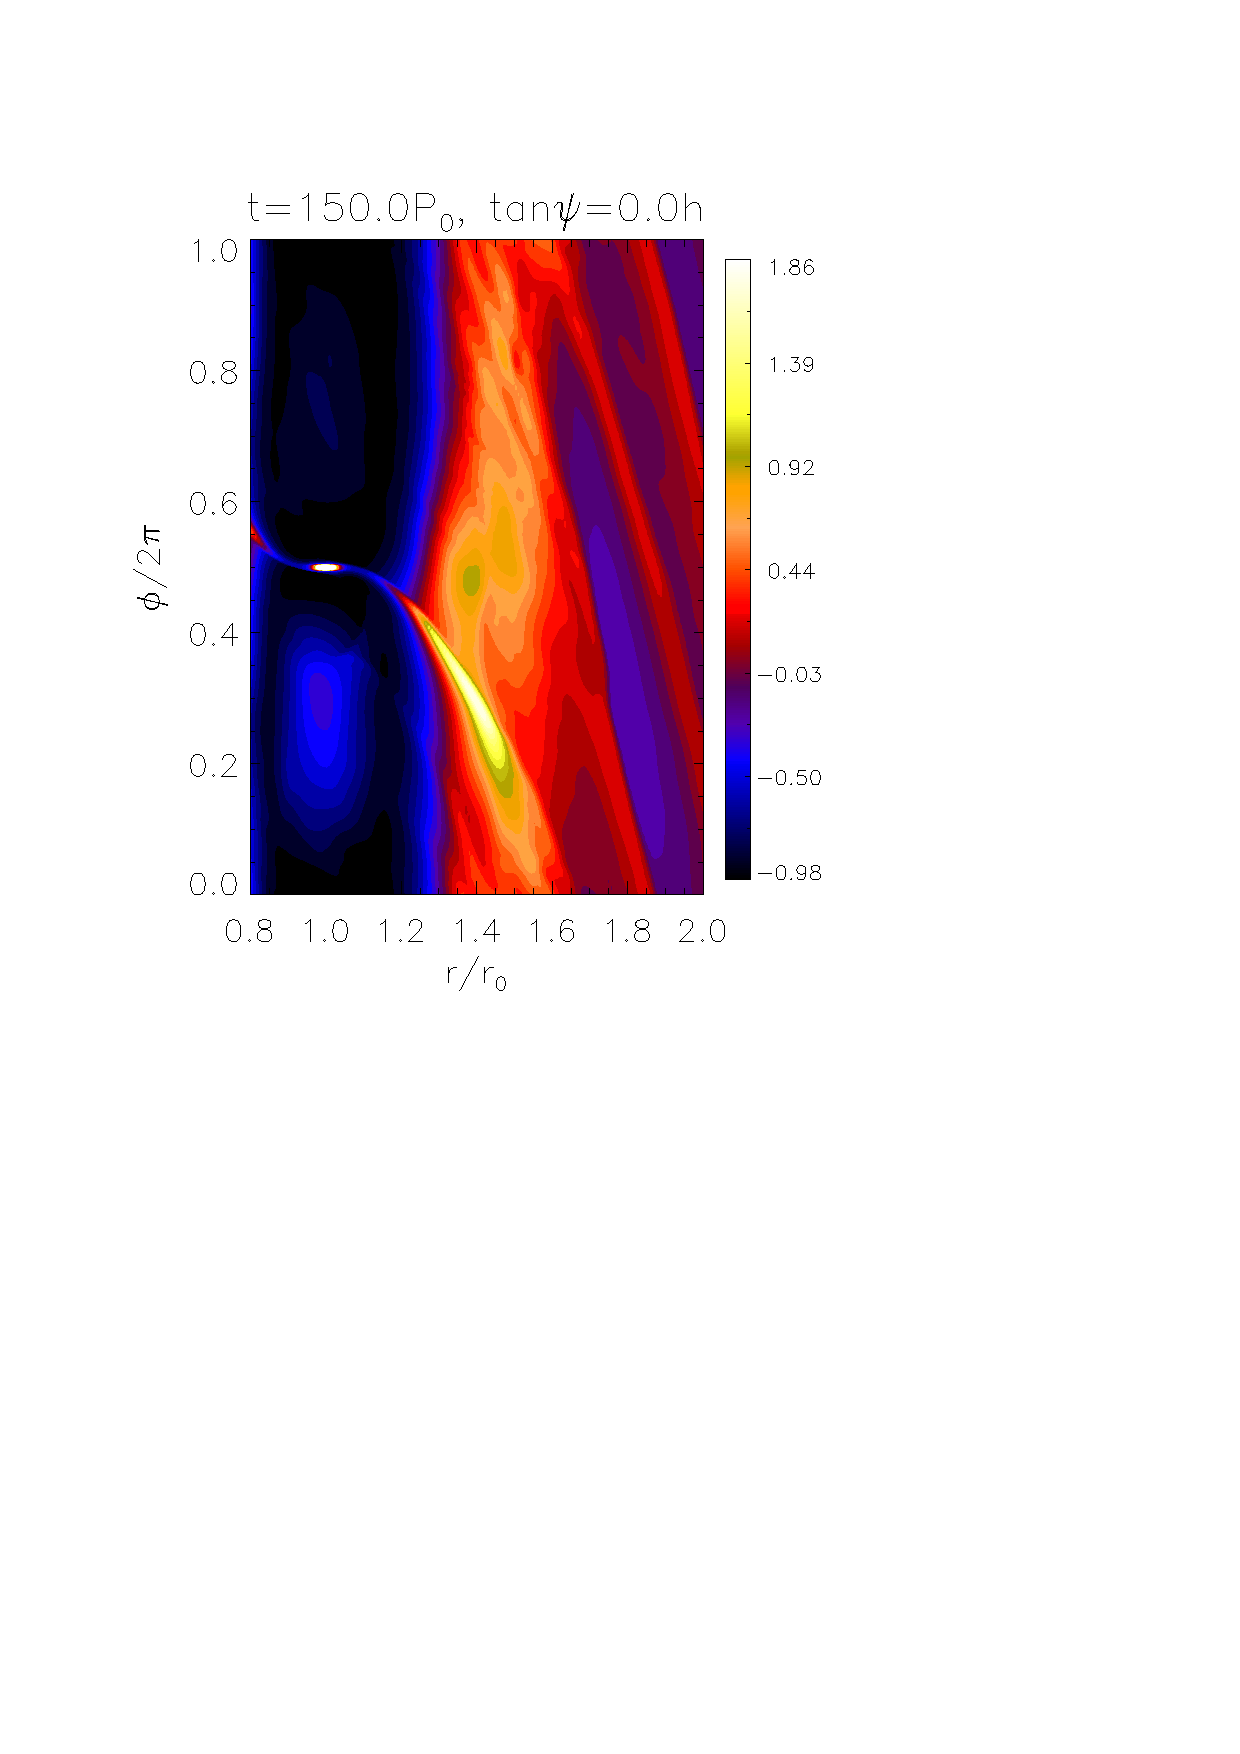
\includegraphics[scale=.43,clip=true,trim=2.3cm
    0.cm 0cm 0.9cm]{figures/jup1_3h_pdisk_015}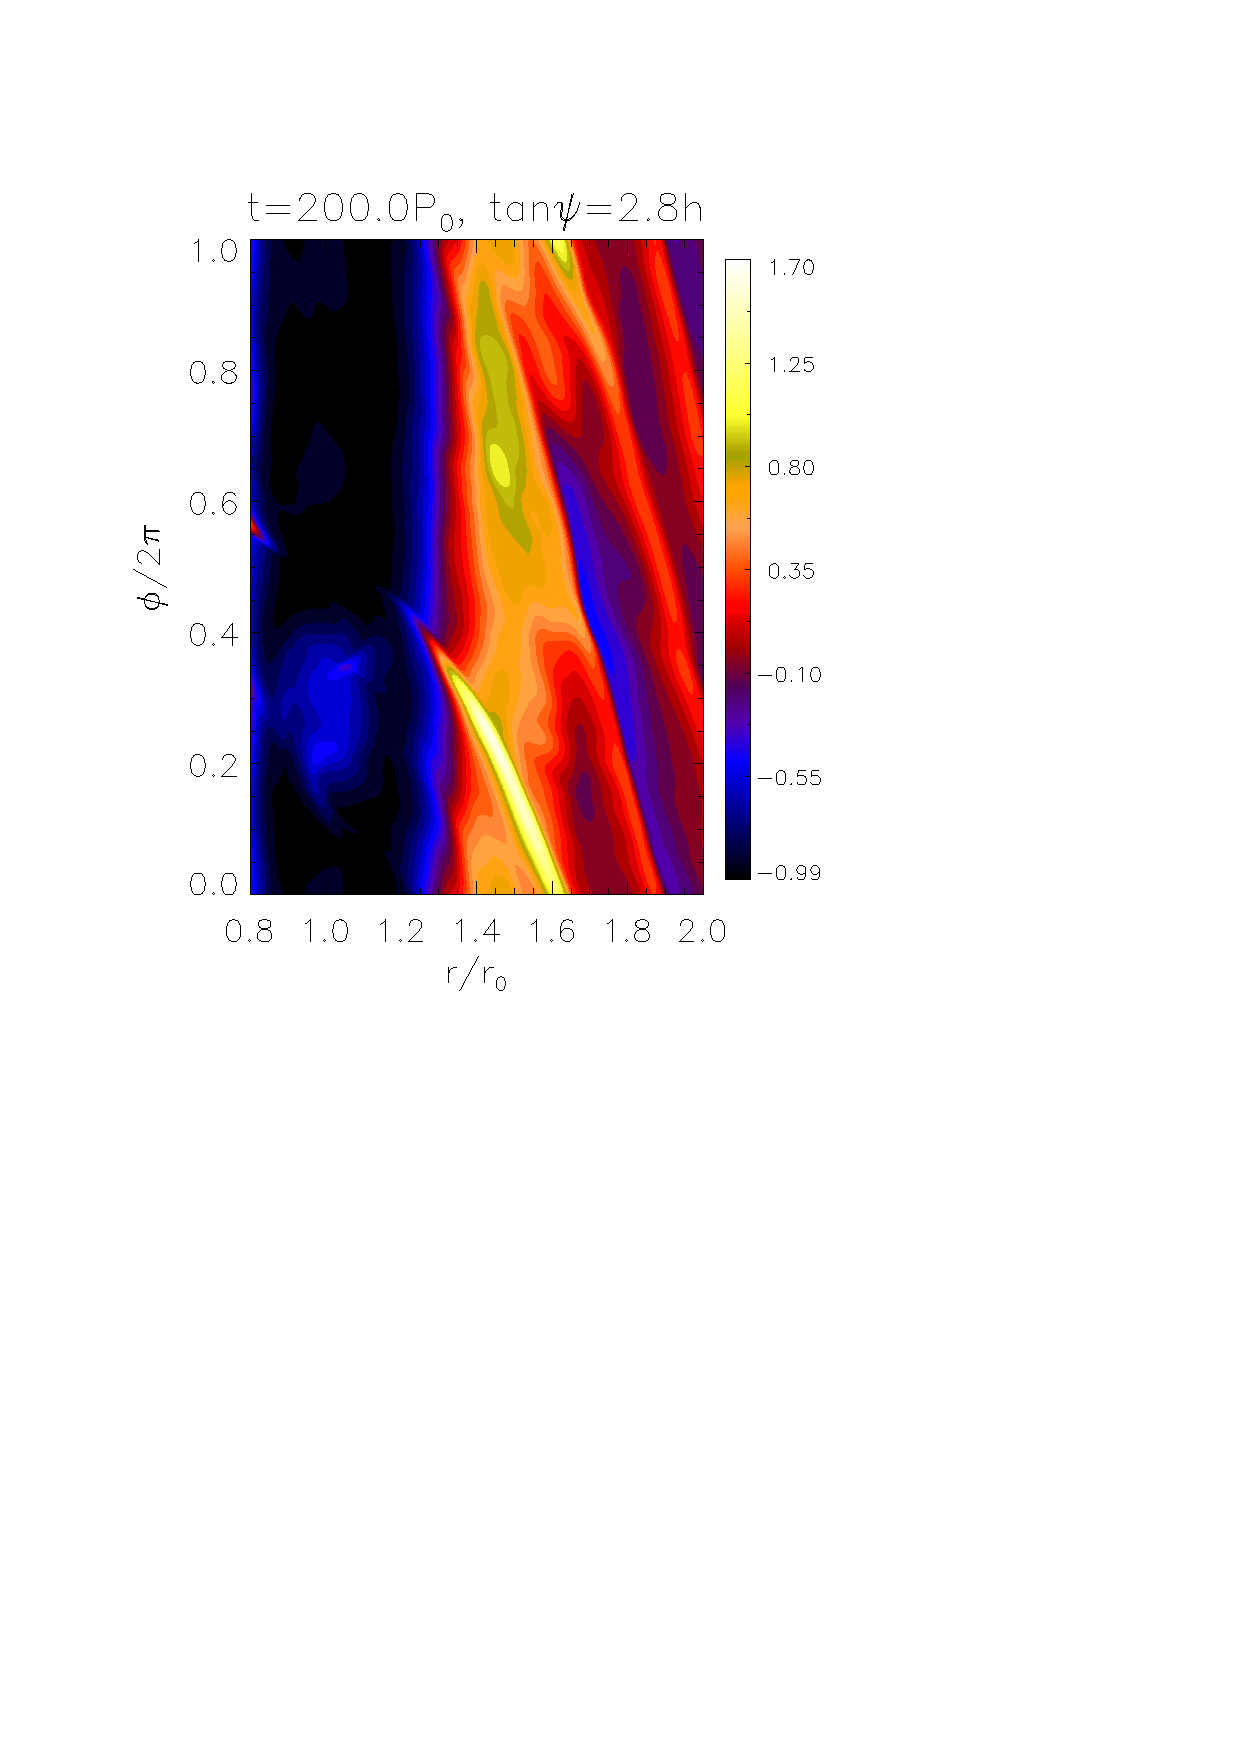
\includegraphics[scale=.43,clip=true,trim=2.3cm
    0.cm 0cm 0.9cm]{figures/jup1_3h_pdisk_020}\\
  %    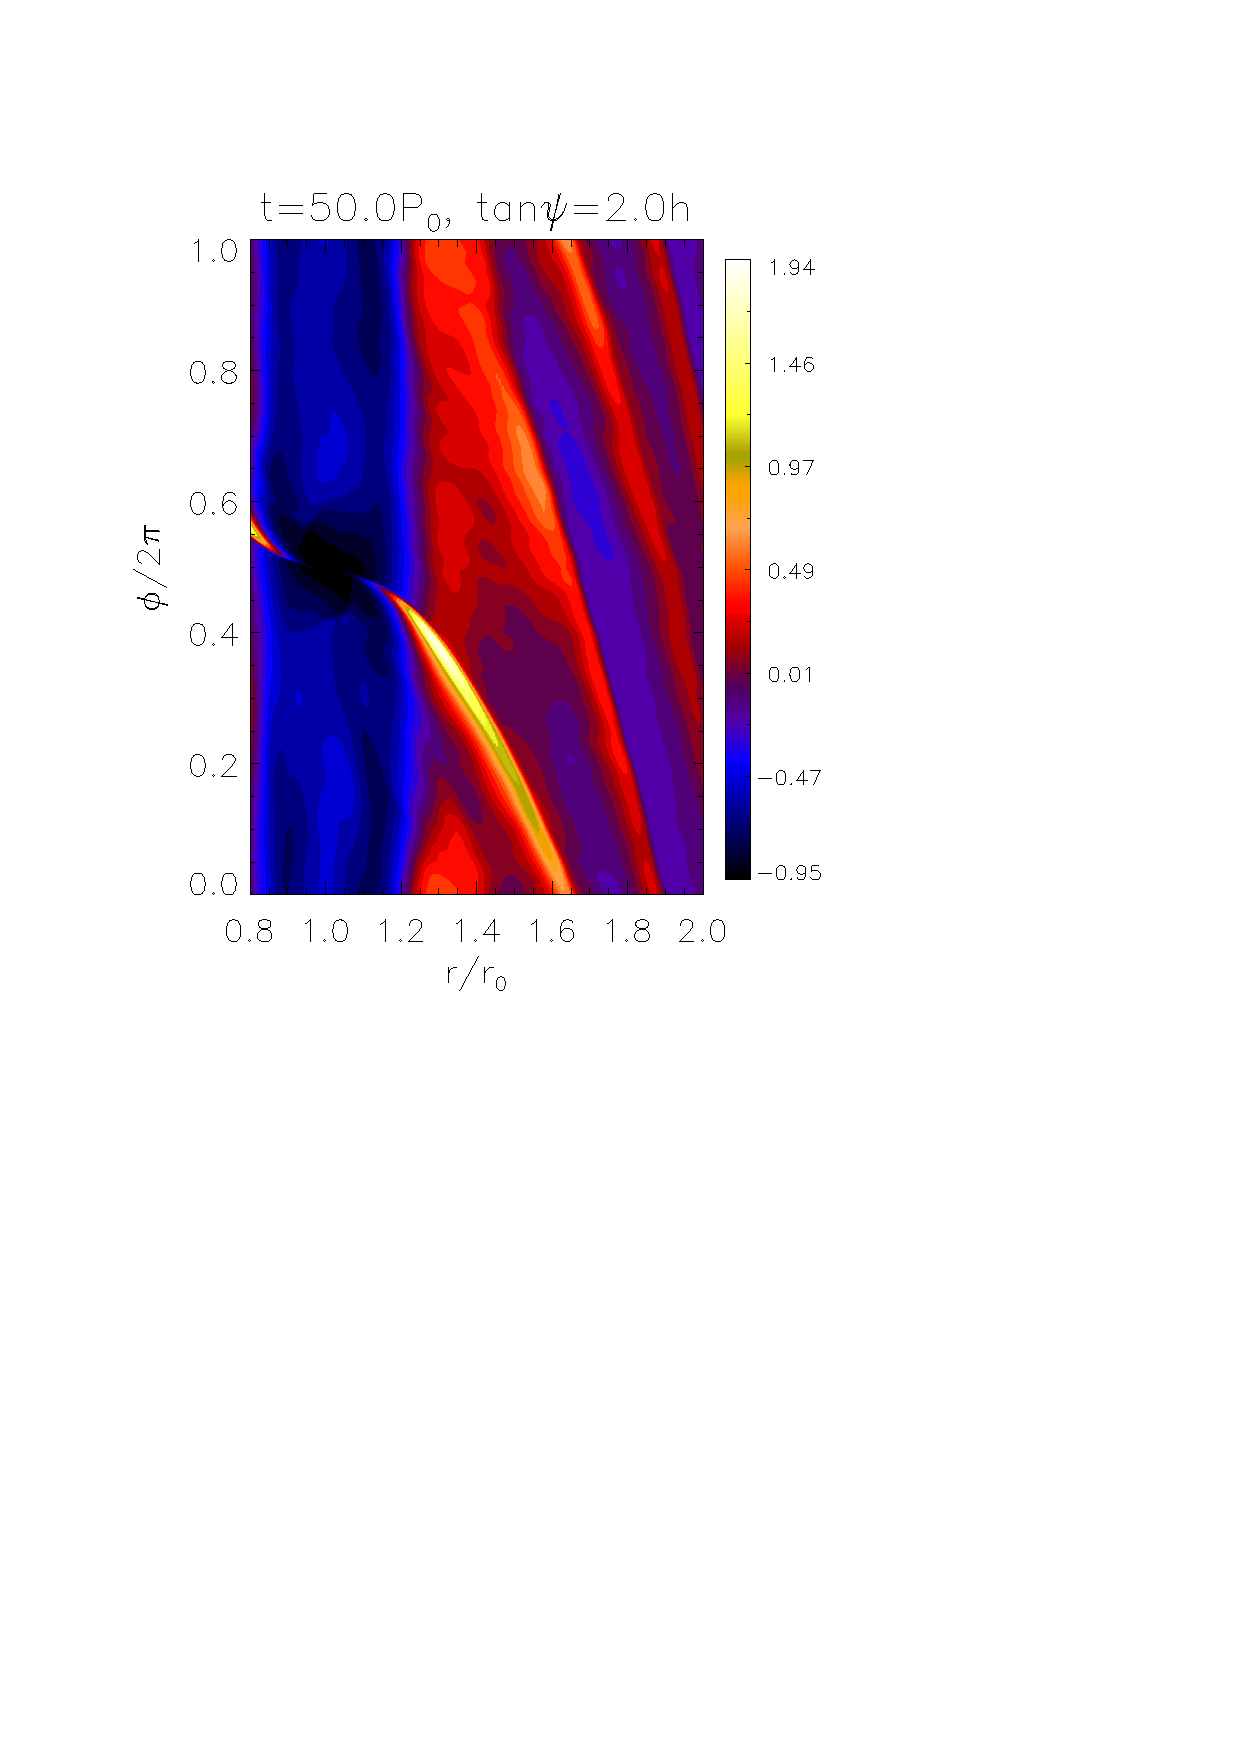
\includegraphics[scale=.43,clip=true,trim=0cm 0.cm 0.cm
  %     0.9cm]{figures/jup2_3h_pdisk_005}
  \caption{Relative density perturbation $\delta\rho$ for disc-planet
    simulations. Top: case P0 (no viscous layer). Bottom: case P1 (viscous layer of $H$). The
    vertical extent of the computational domain is $3H$ and the
    viscous layer is measured from the upper disc boundary.  
    \label{jup0_3h}}
\end{figure*}

\subsubsection{Kinetic energy density}%prob replace with nu_floor=1d-6,
                                %amp=10 sims
Here, we compare the $m=1$ component of the kinetic energy density
($W_1$)  between the no-layer case P0, layered
case P1 and case P0R which is case P0 resumed from $t=100P_0$ with a
viscous layer. Fig. \ref{pdisk_kerz_cases_planet} shows 
$W_1(t)$ averaged over the outer gap edge. For each case we
average $W_1$ over the disc bulk and the atmosphere, and plot them
separately in the figure. 

The $m=1$ component does not emerge from the linear instability, but is a
result of non-linear vortex merging. 
Fig. \ref{pdisk_kerz_cases_planet} shows that merging is accelerated
by a viscous layer: the single vortex appears at $t\sim70P_0$ for case
P1 but only forms at $t\sim120P_0$ for case P0. Also note for all
cases, $W_1$ in the disc bulk (thick lines) is similar to that in the
disc atmosphere (thin lines), implying the $m=1$ disturbance
(i.e. the vortex) evolves two-dimensionally. We checked that this is
consistent with the Froude number $Fr\equiv|Ro|H/z < 1 $ away from the
midplane \citep{barranco05,oishi09}. 

%check froud number is
%less than 1

Case P0R shows that introducing a viscous layer eventually destroys
the vortex. The local viscous timescale $t_\nu\equiv
H^2/\nu\gtrsim 16P_0$ so on short timescales after introducing the 
viscous layer ($t=100P_0$), vortex-merging proceeds in case P0R
similarly to case P0 ($t\in[100,110]P_0$). However, $W_1$ decays for
$t>110P_0$ and evolves towards that of case P1. We expect viscosity
to damp the $m=1$ disturbance in the disc atmosphere between
$t\in[110,200]P_0$ because this corresponds to $\sim 6 t_\nu$, but 
the disturbance in the disc bulk is also damped out: the evolution
remains two-dimensional.    

\begin{figure}
  \centering
  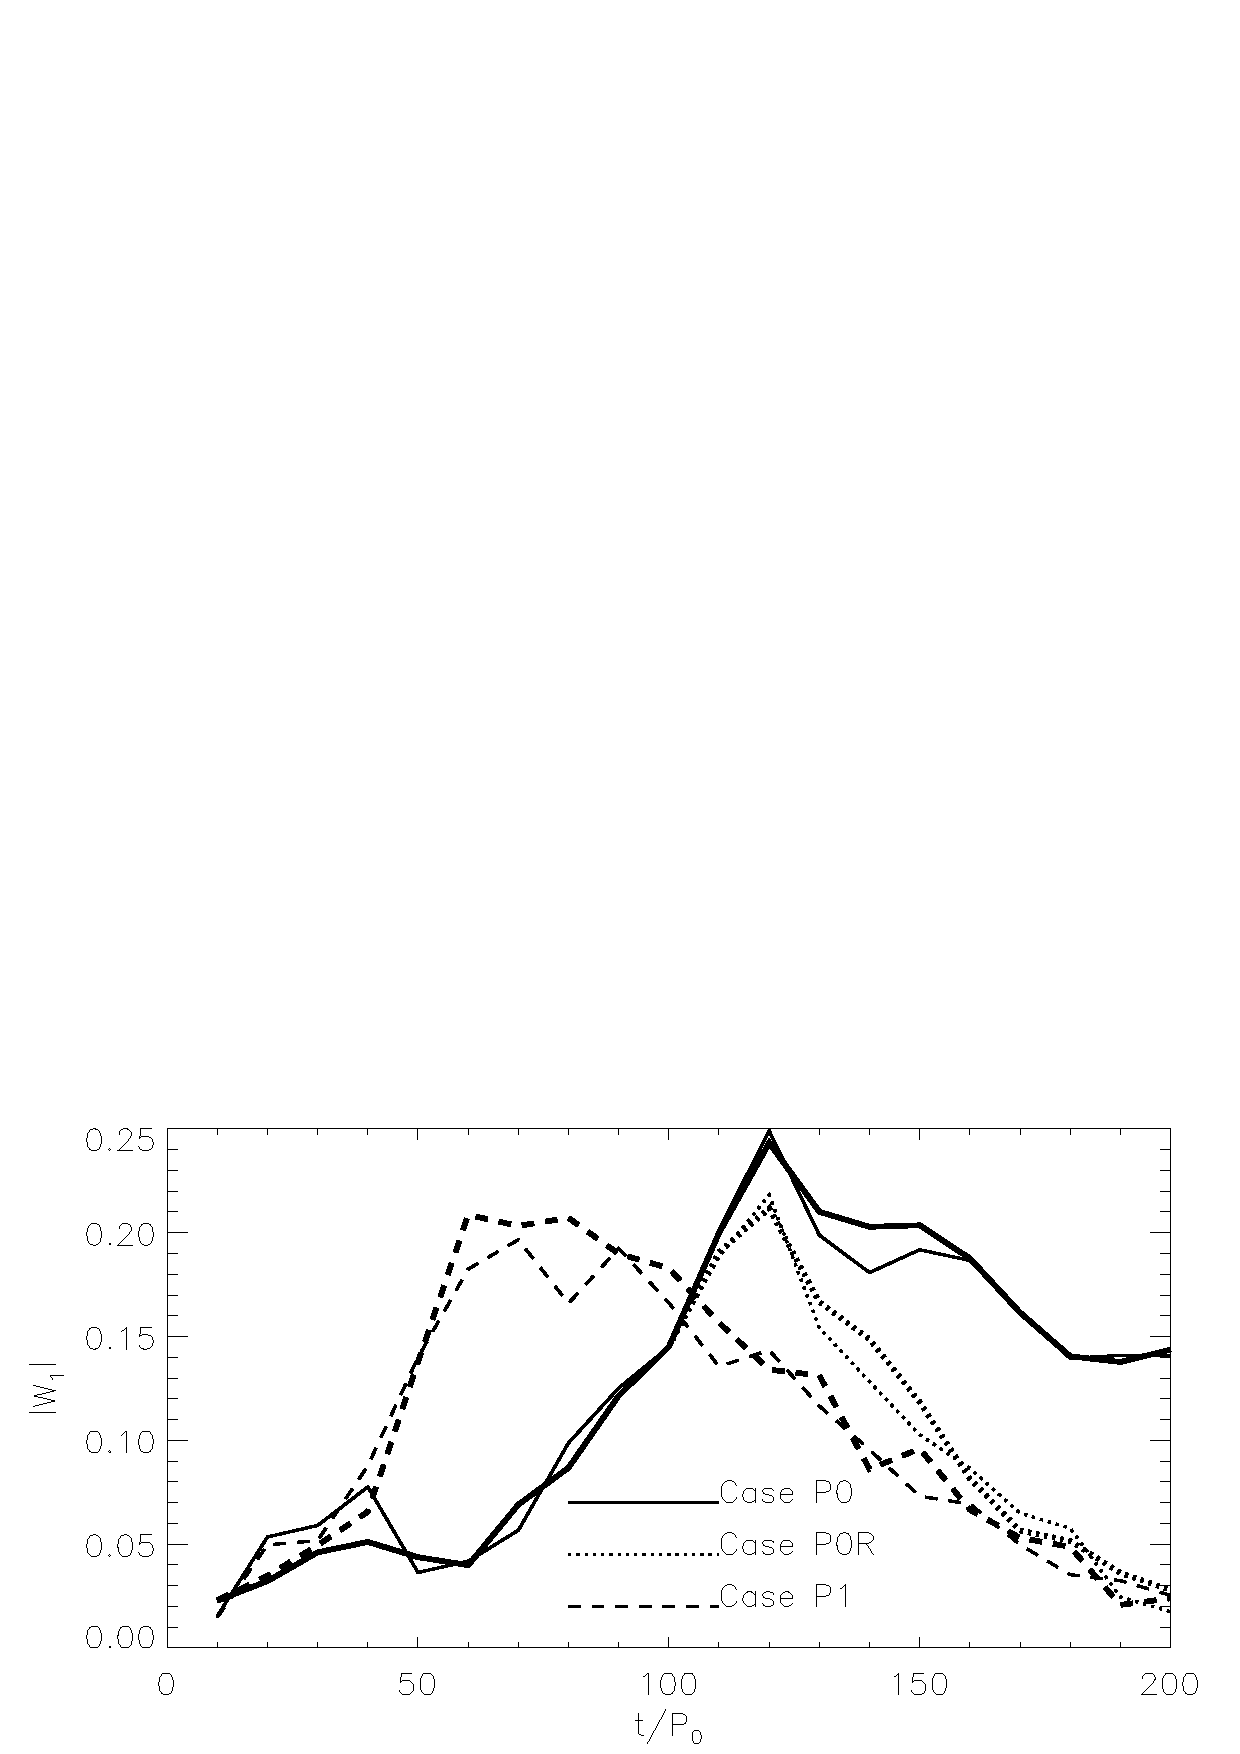
\includegraphics[width=\linewidth]{figures/pdisk_kerz_cases_planet_m1}
  \caption{Evolution of the $m=1$ component of kinetic energy density,
    averaged over $r\in[1.2,1.6]r_0$. This average
    is split into that taken over disc bulk ($z\in[0,2]H$, thick
    lines) and the disc atmosphere ($z\in[2,3]H$, thin lines). Case P0
    has no viscous layer (solid) and case P1 has a viscous layer in
    $z\in[2,3]H$ (dashed). Case P0R is identical to case P0 up to $t=100P_0$,
    but was simulated with a viscous layer of thickness
    $H$ for $t>100P_0$. 
\label{pdisk_kerz_cases_planet}}
\end{figure}

We emphasize the kinetic energy is dominated by horizontal
motions, with $\mathrm{max}(|v_z|/|\bm{v}|) < 0.03$ at the outer
gap edge ($r\in[1.2,1.6]r_0$). Vertical motions are well sub-sonic. When averaged
over $z\in[0,2]H$ and $z\in[2,3]H$, the vertical Mach number
$M_z\equiv|v_z|/c_s=0.05,\,0.08$ (P0), $M_z=0.04,\,0.05$ (P0R) and
$M_z=0.05,0.06$ (P1), respectively. That is, $|v_z|$
increases with height, but the difference between $v_z$ in the disc
atmosphere and that near the midplane diminishes when viscosity is
present in the former. 

\subsubsection{Potential vorticity}
We examine the PV evolution for case P0R in
Fig. \ref{jup0_3h_visc_restart_vorten}, but  
to highlight the vortices, which are positive (negative)
density (vertical vorticity) perturbations, we show the inverse PV
perturbation, $\eta_z(t=0)/\eta_z - 1$. As noted above, a single vortex still forms
despite introducing a viscous layer at $t=100P_0$. However, this
vortex decays rapidly compared to case P0. The vortex elongates, 
producing a `tail' ($t=160P_0$), and eventually the vortex core
disappears altogether.  


\begin{figure*}
  \centering
  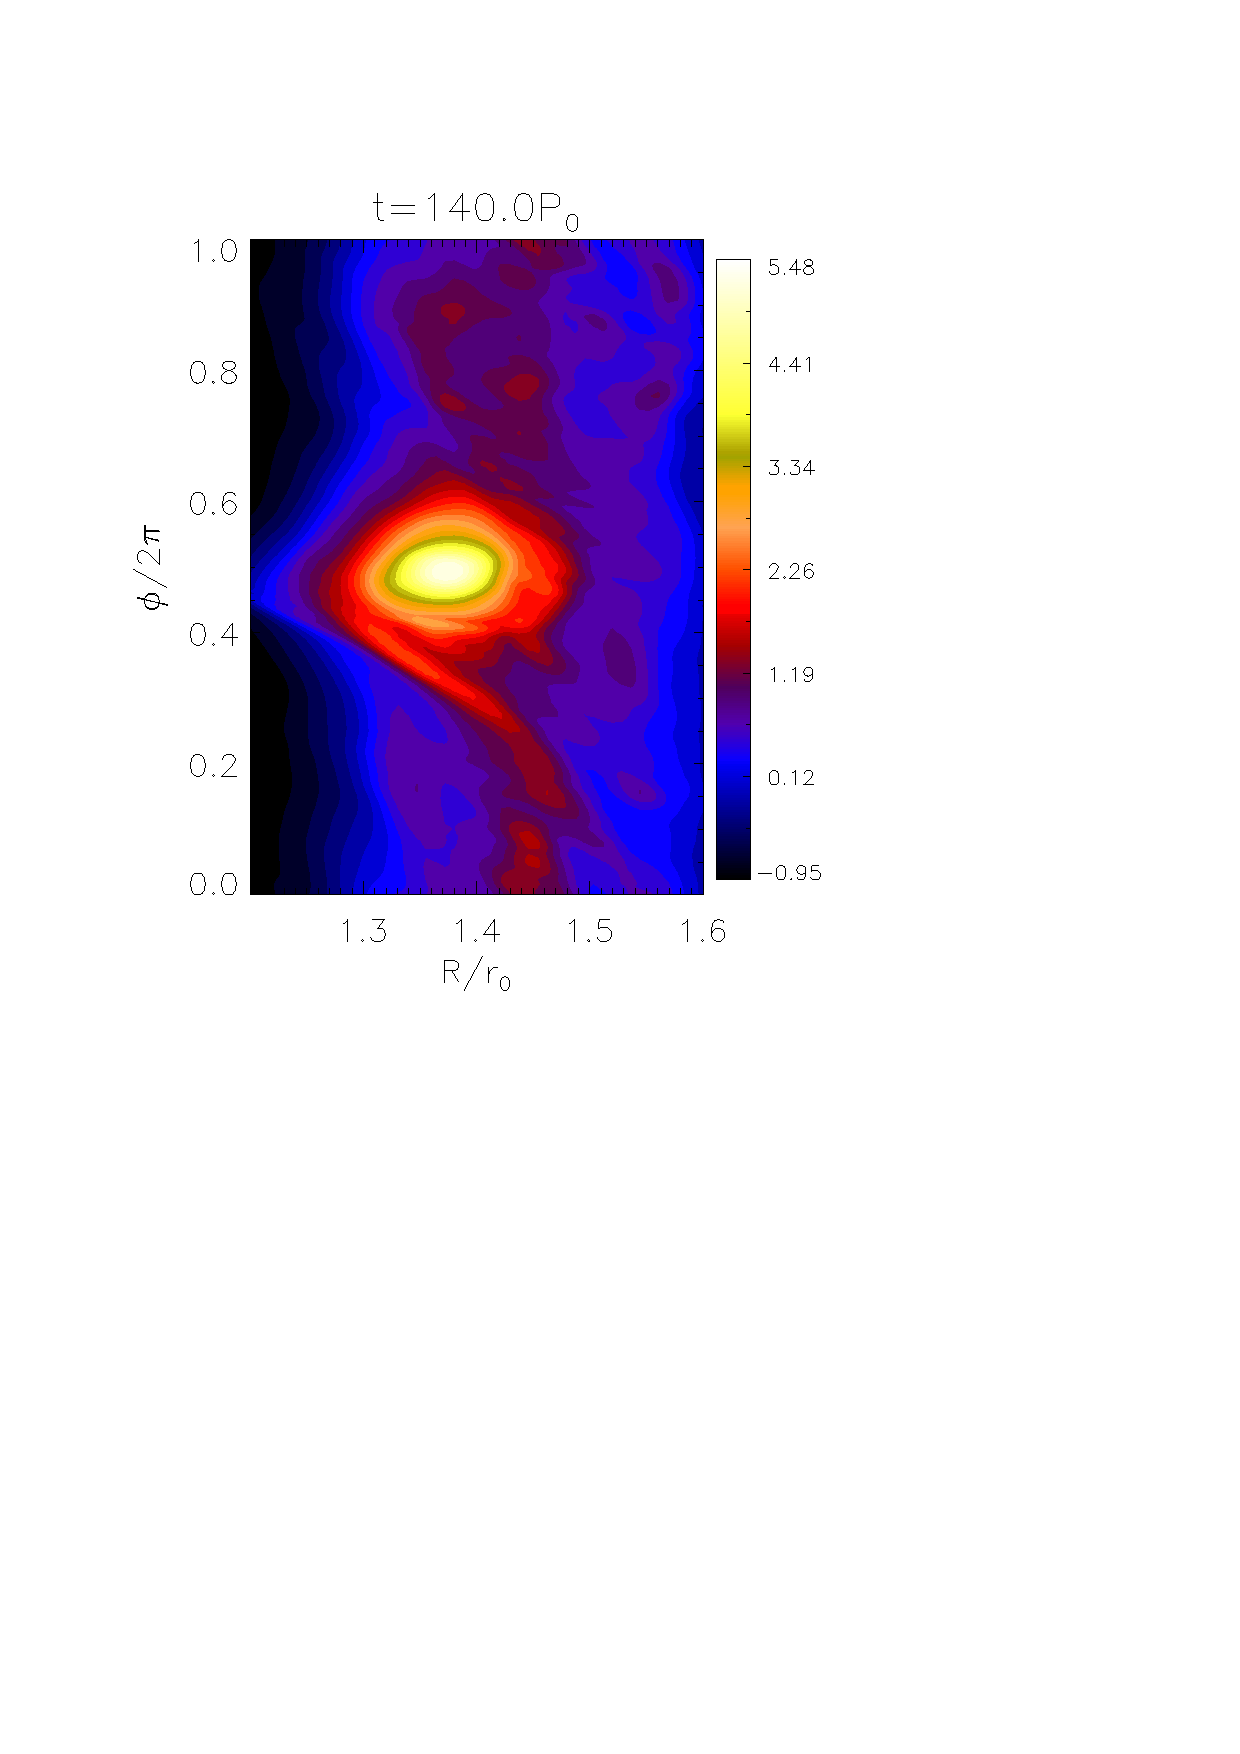
\includegraphics[scale=.43,clip=true,trim=0cm .0cm 0cm
    0cm]{figures/jup0_3h_visc_restart_pdisk_vorten_014}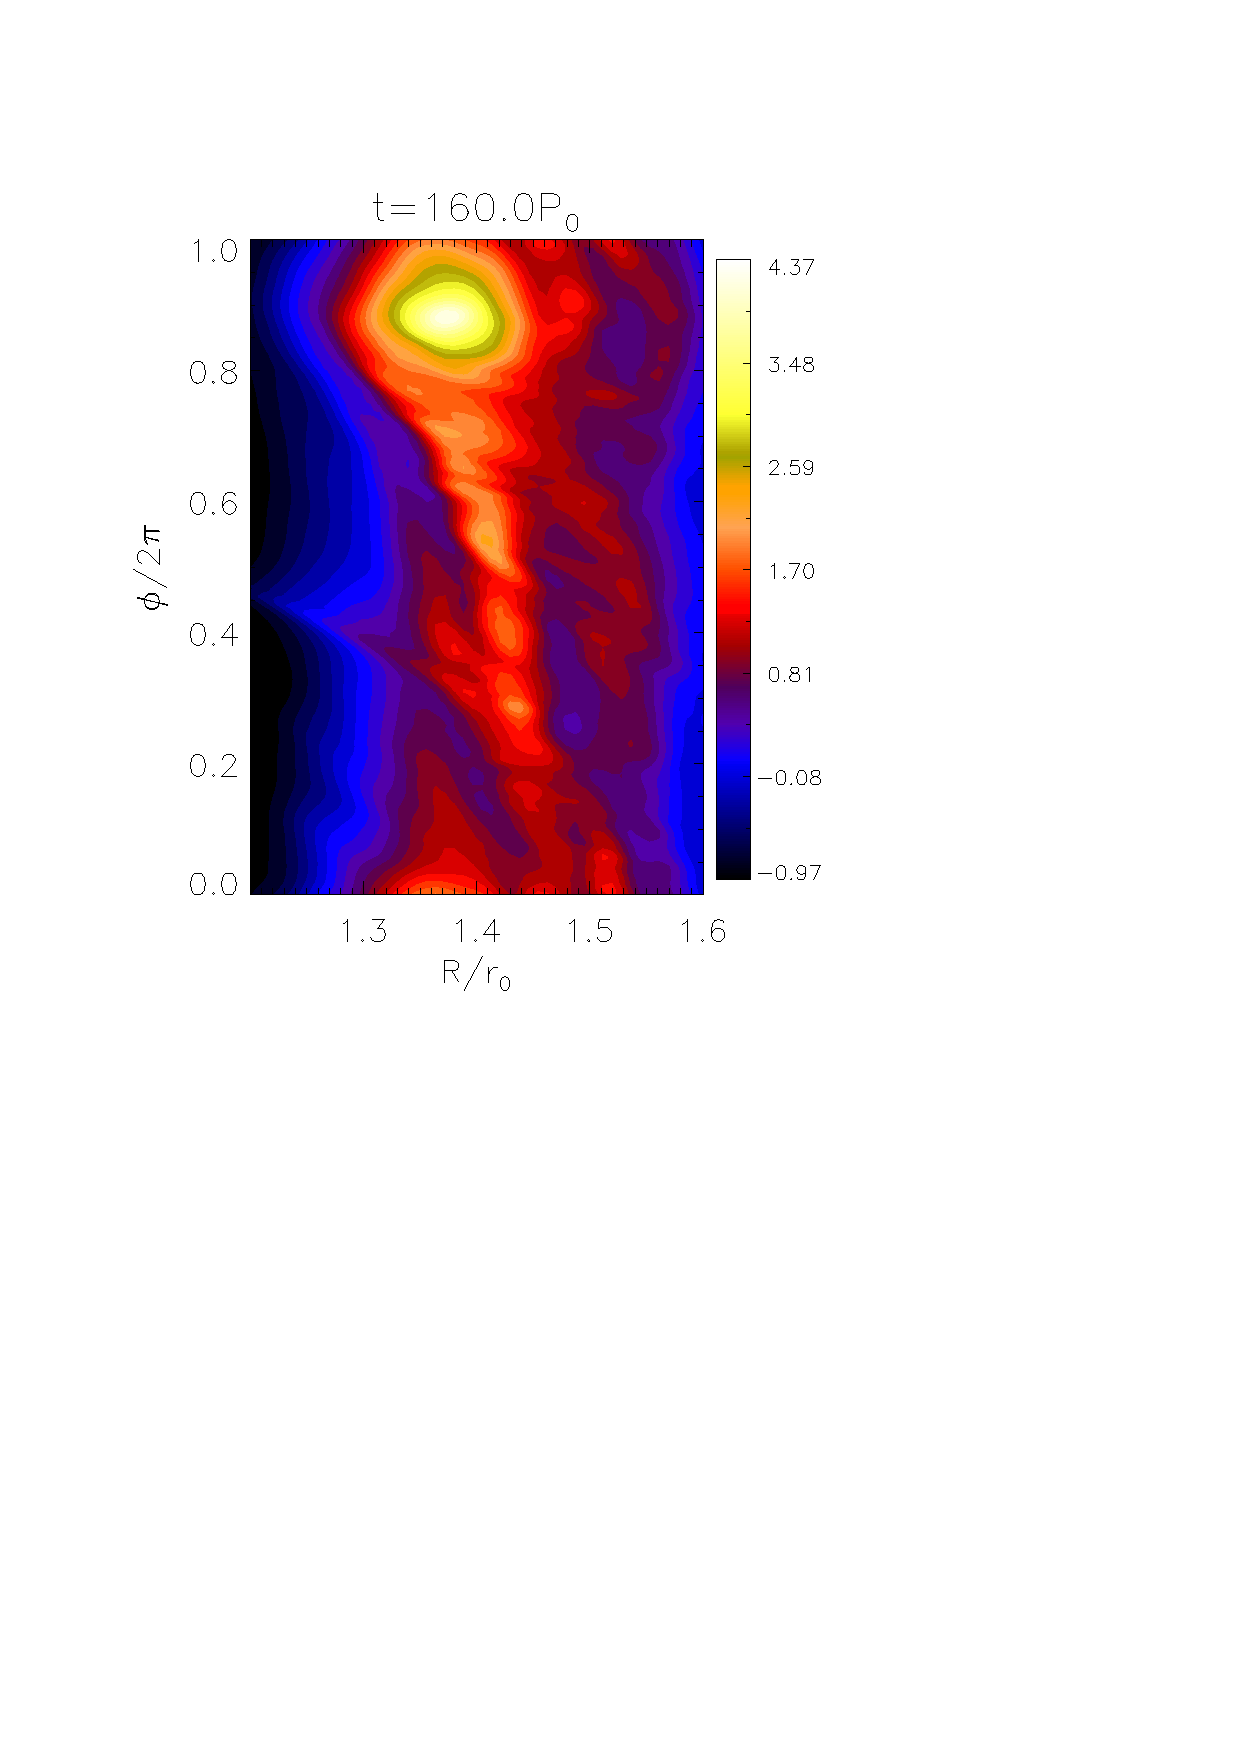
\includegraphics[scale=.43,clip=true,trim=2.3cm
    .0cm 0cm 0cm]{figures/jup0_3h_visc_restart_pdisk_vorten_016}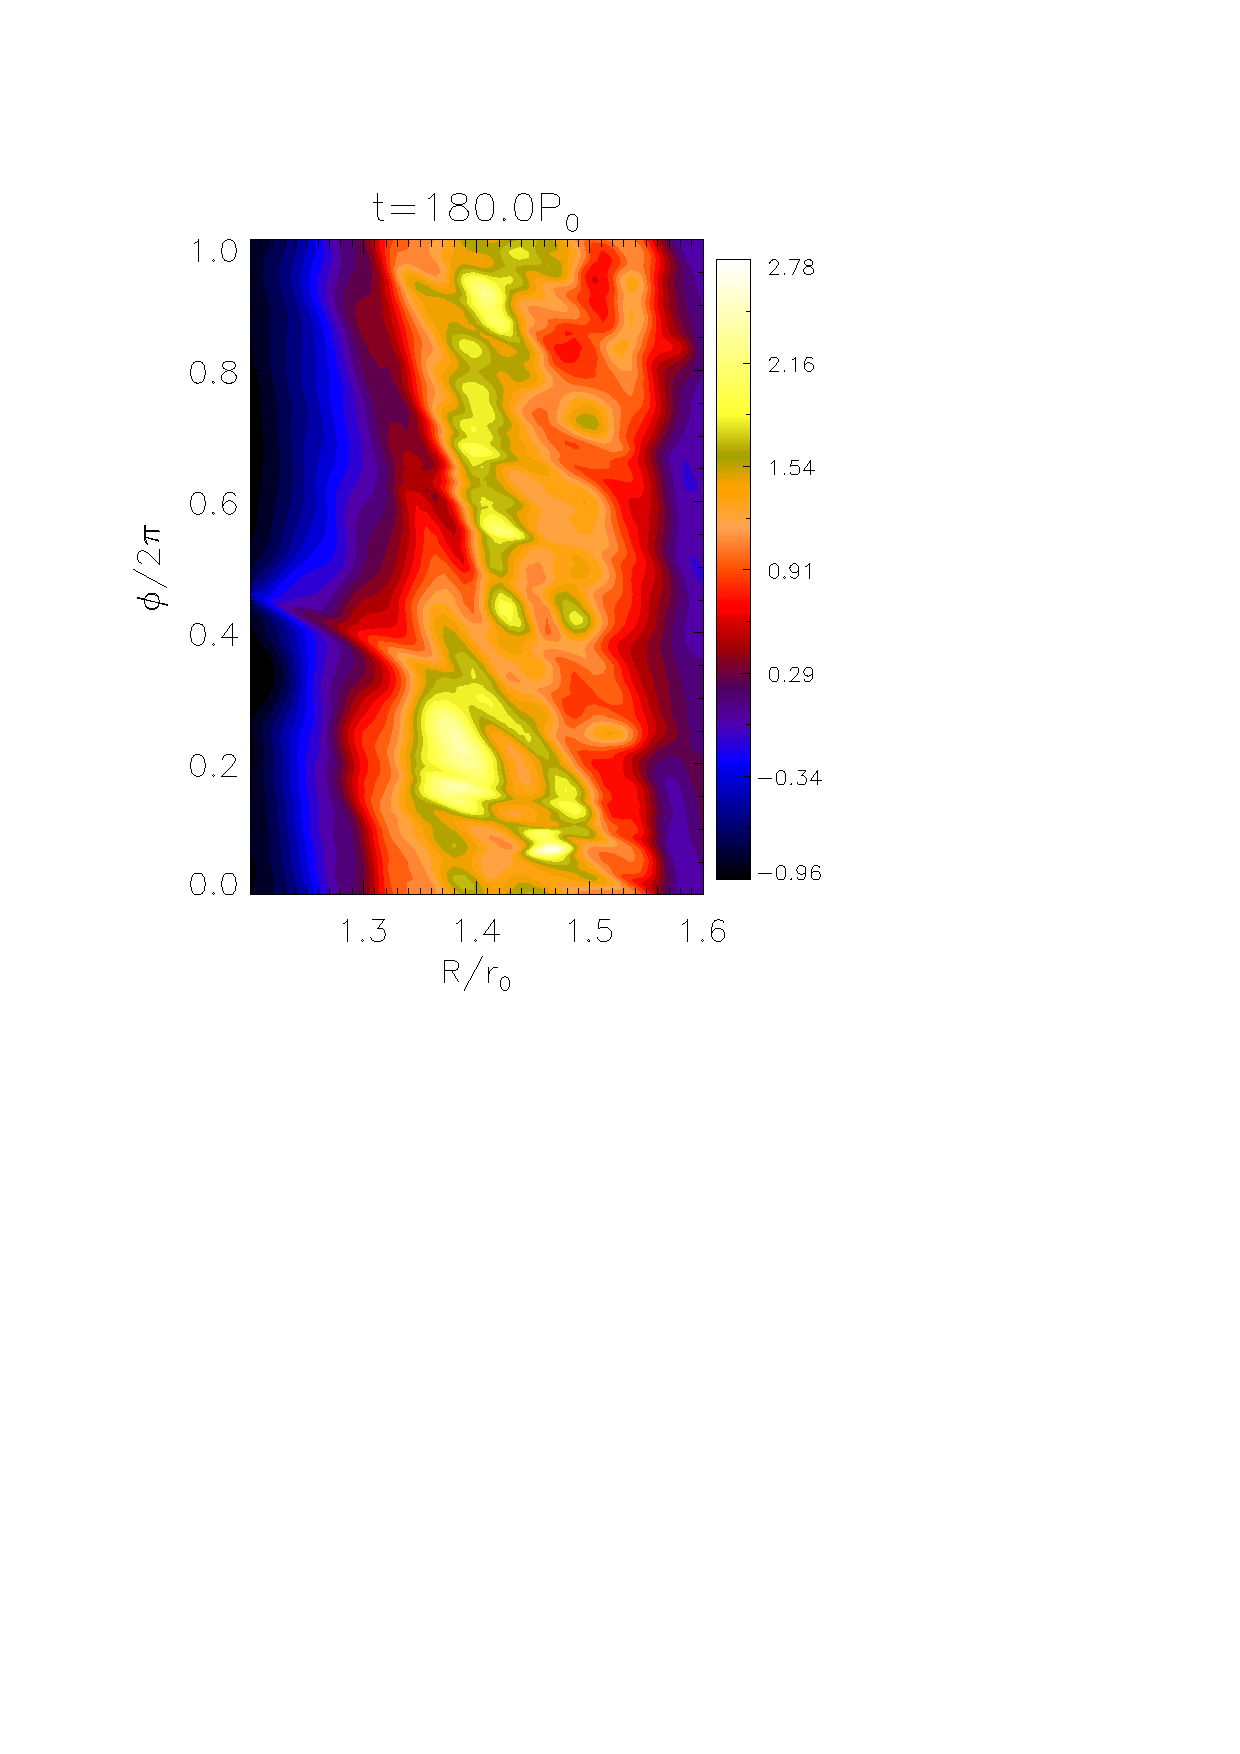
\includegraphics[scale=.43,clip=true,trim=2.3cm
    .0cm 0cm 0cm]{figures/jup0_3h_visc_restart_pdisk_vorten_018}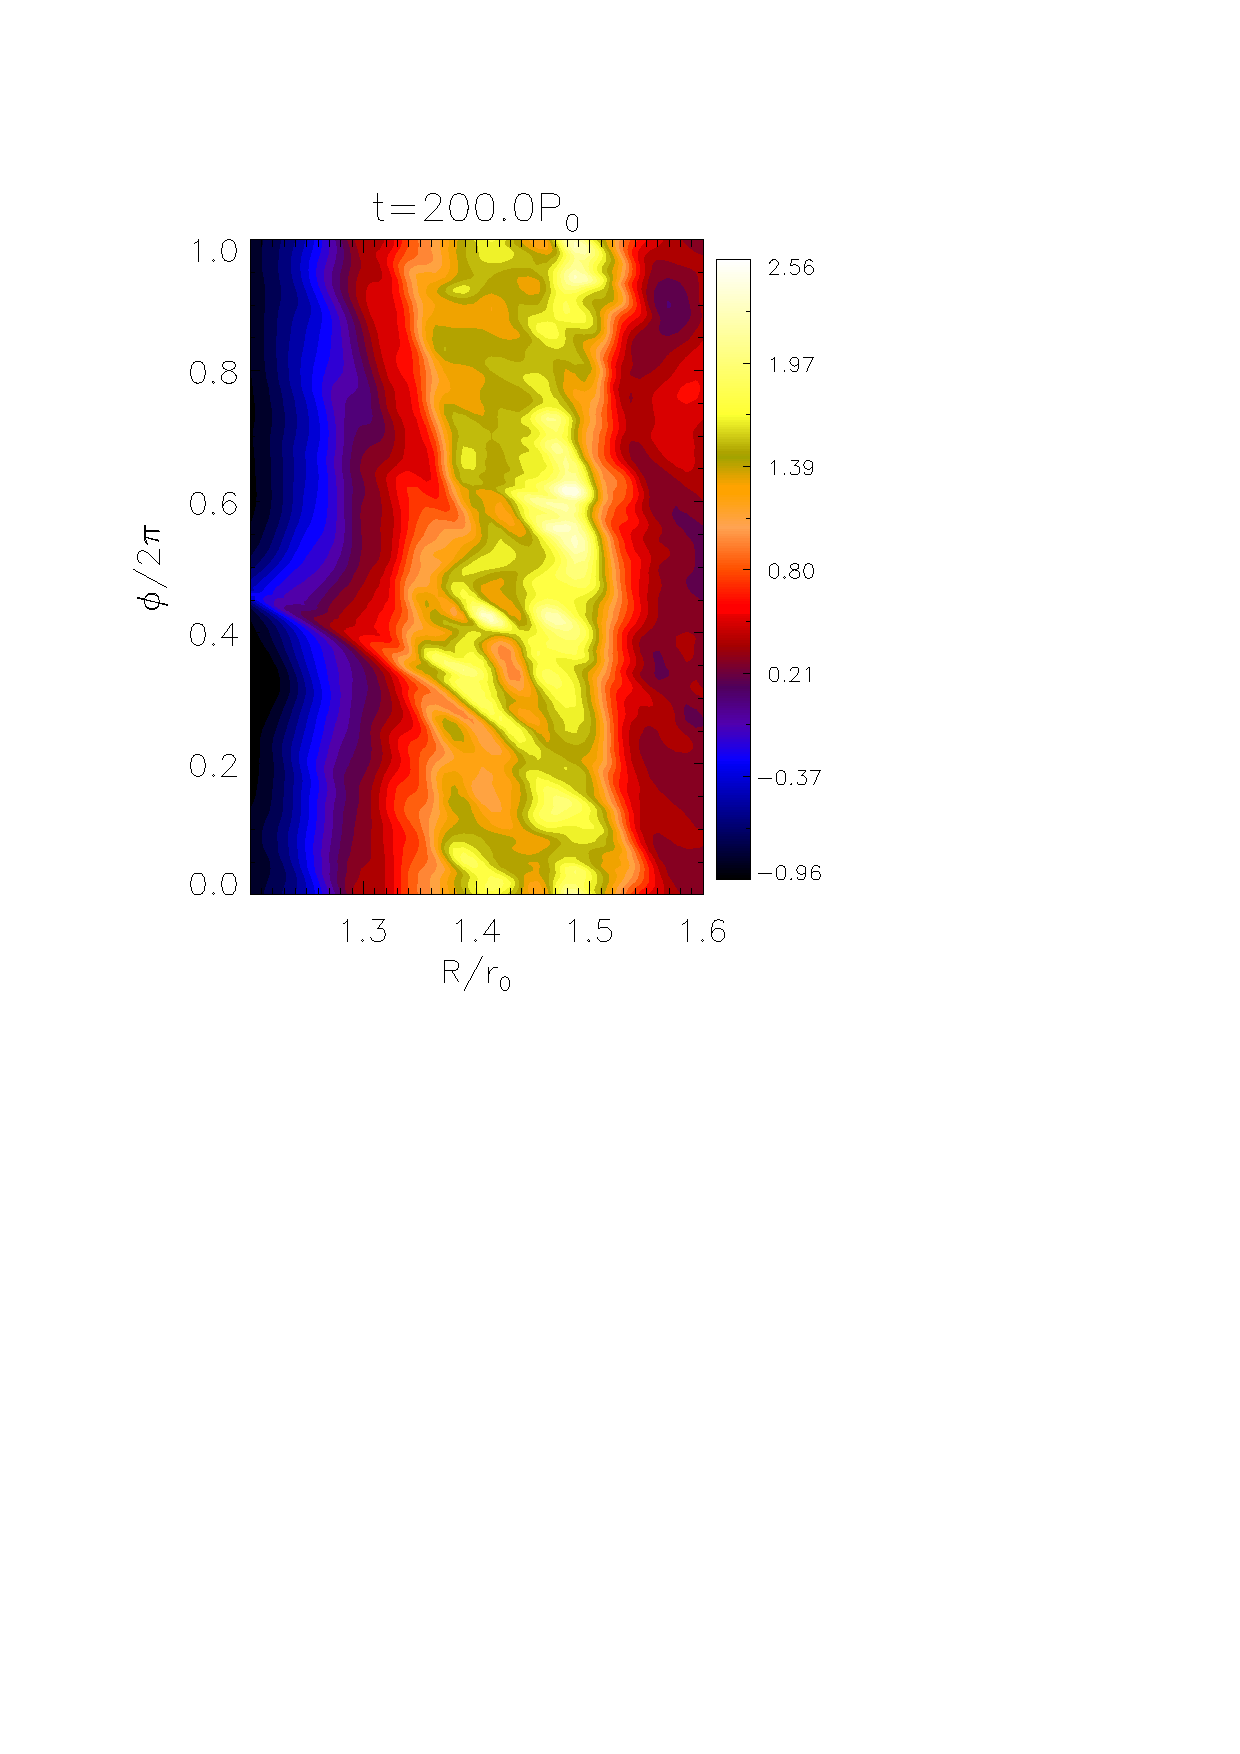
\includegraphics[scale=.43,clip=true,trim=2.3cm
    .0cm 0cm 0cm]{figures/jup0_3h_visc_restart_pdisk_vorten_020}
  \caption{Inverse PV perturbation for case P0R, which was resumed
    from the no-layer case P0 from $t=100P_0$ with the introduction of
    a viscous layer of $H$. 
    \label{jup0_3h_visc_restart_vorten}}
\end{figure*}

\subsubsection{Resolution check}%prob just commentary
We repeated simulations P0 and P1 with resolution
$(N_r,N_\theta,N_\phi)=(512,96,1536)$, corresponding
to $12$ and $32$ cells per scale-height in $(r,\phi)$ and $\theta$,
respectively. We denote these runs as P0HR and P1HR below. 

We observe similar evolution in P0HR and P1HR as their standard
resolution versions. However, due to lower numerical diffusion, we
find stronger vortices in P0HR. Although the vortex in P1HR persisted
longer than the standard resolution run, it was still subject to rapid
decay in comparison with P0HR. At $t=200P_0$ we find 
the $m=1$ amplitude to be $a_1=0.29$ and $a_1=0.10$ at the outer gap
edge, respectively for P0HR and P1HR; a similar contrast as that
between P0 and P1. A weak over-density was still observed in
P1HR, but it further decays to $a_1=0.06$ at $t=230P_0$ and a vortex is
effectively absent. By contrast, P0HR was simulated to $t=250P_0$ and
the vortes survived with $a_1=0.25$.   

   

%Interestingly, we observe small-scale instability inside the
%vortex. This is shown in Fig. . We suspect this is the elliptic
%instability, but cannot prove this. It is absent in P1HR.  

\subsection{Additional simulations}% higher visc, strict isothermal 
Locally isothermal, low viscosity discs are vulnerable to the
so-called `vertical shear 
instability' because $\partial_z\Omega_i\neq 0$ \citep{nelson12}. 
\citeauthor{nelson12} employed a radial  resolution $\gtrsim 60$ cells
per $H$ to resolve this instability because it involves small radial
wavelengths ($\ll H$). Our numerical resolution is unlikely to capture
this instability. Nevertheless, we have performed additional
simulations designed to eliminate the vertical shear instability.   

\subsubsection{Larger floor viscosity}
We performed several simulations with $\hat{\nu}_0=10^{-6}$. A viscosity of
$\hat{\nu}\sim 10^{-6}$ is expected to damp the vertical shear 
instability \citep{nelson12}, while still permitting the gap-edge
RWI. Table \ref{planet_sims} summarizes
these cases with $A_\nu=10$ (`Pb' runs) and $A_\nu=100$ (`Pc' runs). 

In these simulations we find vortices eventually decay, even in the
no-layer case Pb0. For $A_\nu=10$, the layered cases Pb0.5 and Pb1 evolve
similarly Pb0: three vortices formed by $t\sim30P_0$, merging into two
vortices by $t\sim40P_0$, then finally into a single vortex by
$t\sim130P_0$, which subsequently decays. However, the final vortex
decays faster in the presence of a viscous layer. This is shown in
Fig. \ref{pdisk_kerz_cases_planet_hivisc}, which compares the $m=1$
kinetic energy density for case Pb0 and Pb1. The evolution only begins
to differ after the single-vortex has formed. 

\begin{figure}
  \centering
  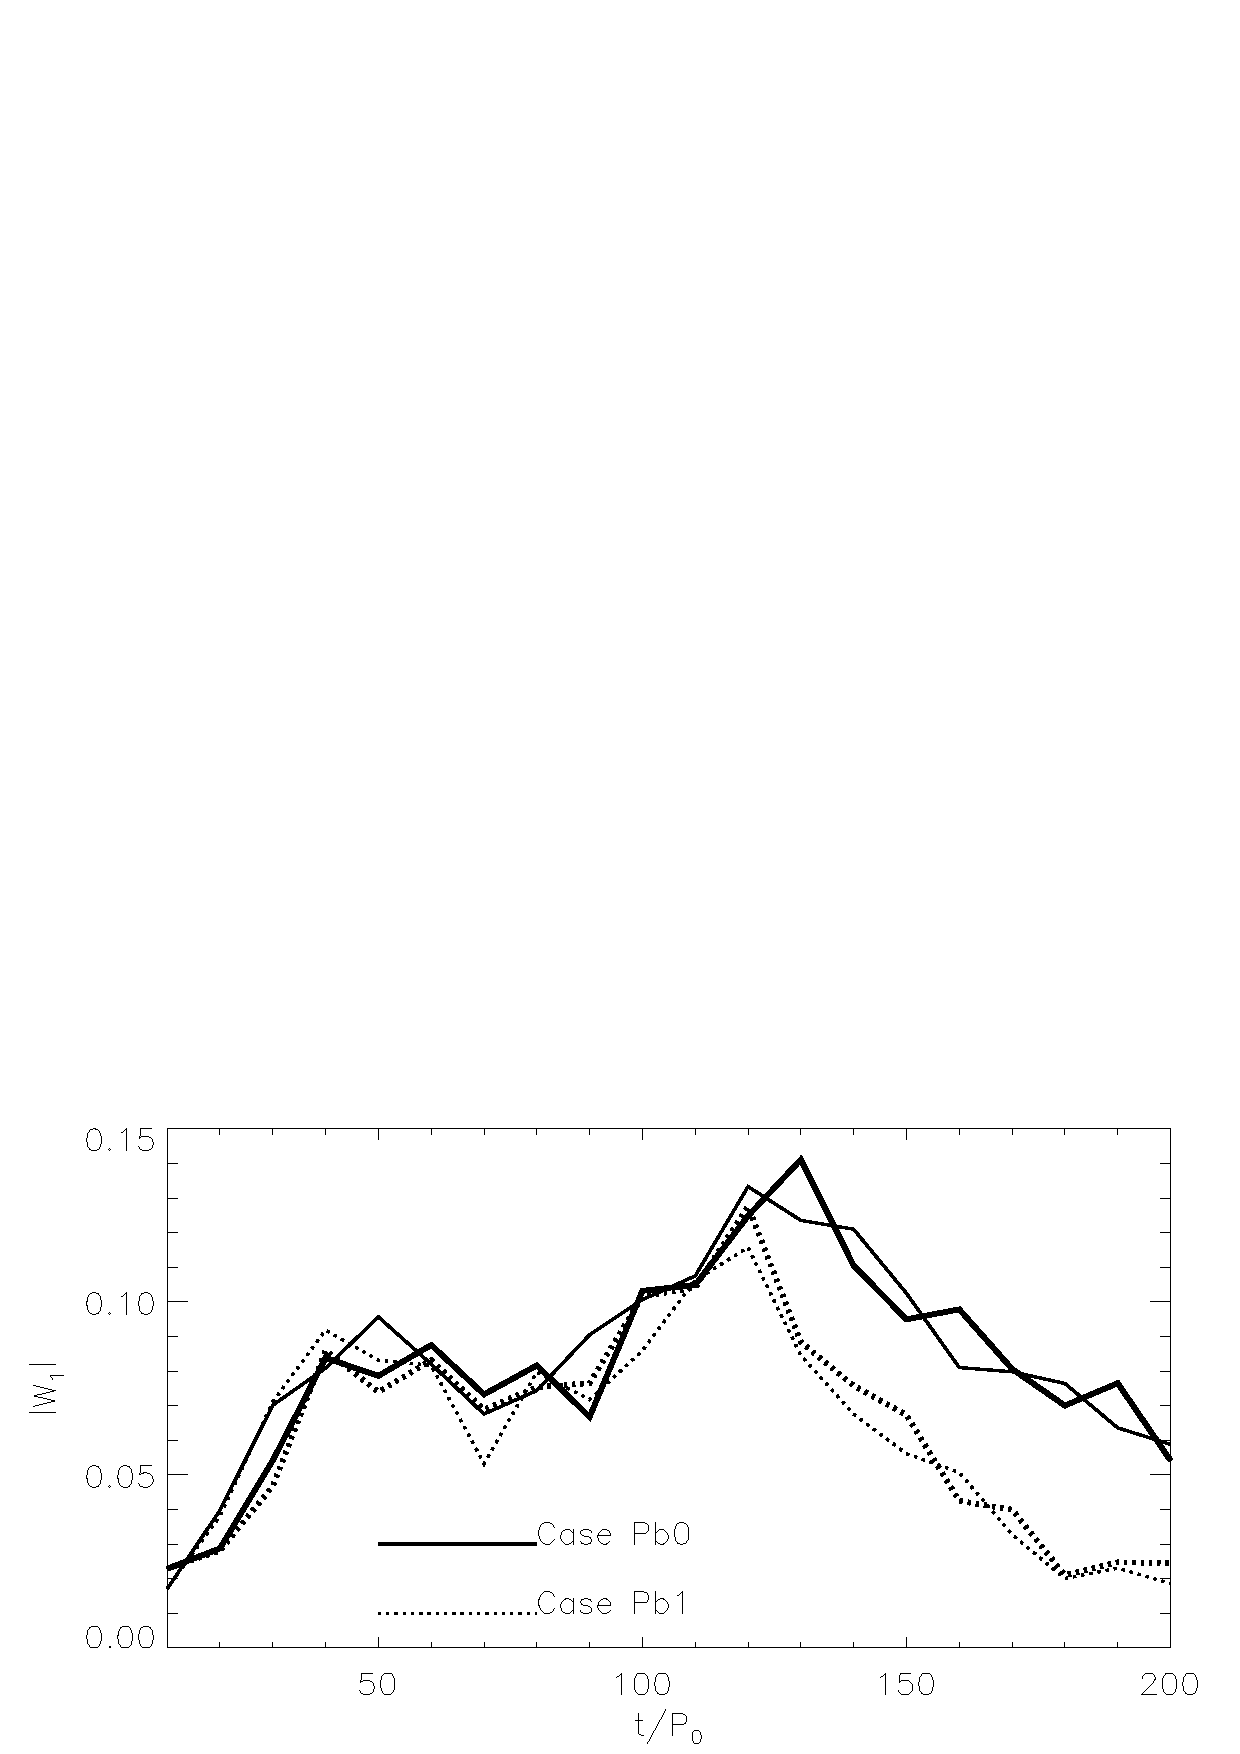
\includegraphics[width=\linewidth]{figures/pdisk_kerz_cases_nu6}
  \caption{Same as Fig. \ref{pdisk_kerz_cases_planet} but with
    floor viscosity $\hat{\nu}_0=10^{-6}$: cases Pb0 (solid, no viscous layer) and Pb1
    (dotted, viscous layer of $H$). The thick (thin) lines indicate
    $W_1$ averaged over $z\in[0,2]H$
    ($z\in[2,3]H$). 
    \label{pdisk_kerz_cases_planet_hivisc}}
\end{figure}


For $A_\nu=100$ (cases Pc0.5 and Pc1), we find the $m=2$ amplitude
dominated over $m=1$, so a single-vortex configuration never
forms. For both Pc0.5 and Pc1 the $m=2$ (two-vortex configuration)
amplitude decreases from $t\sim 50P_0$. For case Pc1, the vortices are
transient features and are entirely absent for $t\gtrsim80P_0$.  


\subsubsection{Strictly isothermal discs} 
We repeated simulations P0, P1 and Q1 with a strictly isothermal
equation of state ($q=0$). These are summarised in Table
\ref{planet_sims_iso}. Fig. \ref{pdisk_kerz_cases_planet_iso} compares
the $m=1$ kinetic energy density for these cases. Consistent with the
above simulations, a viscous layer causes a faster decay in this
quantity. Most interesting though, is that we found case Iso2 (with a viscous
layer of $\sim H$) only shows very weak non-axisymmetric perturbations
early on ($t\lesssim 50P_0$): vortex formation is suppressed. 


%and the end, vortices in all cases?  

\begin{table}
  \centering
  \caption{Disc-planet simulations with a strictly
    isothermal equation of state ($q=0$). The thickness of the viscous layer
    is quoted at the reference radius $R=r_0$. \label{planet_sims_iso}}
    \begin{tabular}{llllrc}
      \hline\hline
      Case & $10^6\hat{\nu}_0$ & $A_\nu$ & visc. layer& $10^2\overline{a}_1$ &vortex \\ 
      \hline
      Iso0   & 1.0  & 1          & 0      & 19.3  &  YES   \\
      Iso1   & 1.0  & 10         & $H_0$  & 12.8  &  YES     \\ 
      Iso2   & 1.0  & 100        & $H_0$  & 1.1  &  NO     \\ 
      \hline
  \end{tabular}
\end{table}

%Fig. \ref{iso_vorten} shows the inverse PV perturbation for isothermal
%disc-planet simulations. Again, in all cases we observe the RWI to
%grow initially (we identified non-axisymmetric disturbances for
%$t\lesssim 50P_0$). These disturbances merge into a single vortex in the
%no-layer case Iso0. However, case Iso2 does not develop the single vortex in
%the non-linear regime: the gap edge becomes axisymmetric and remains
%stable. 


\begin{figure}
  \centering
  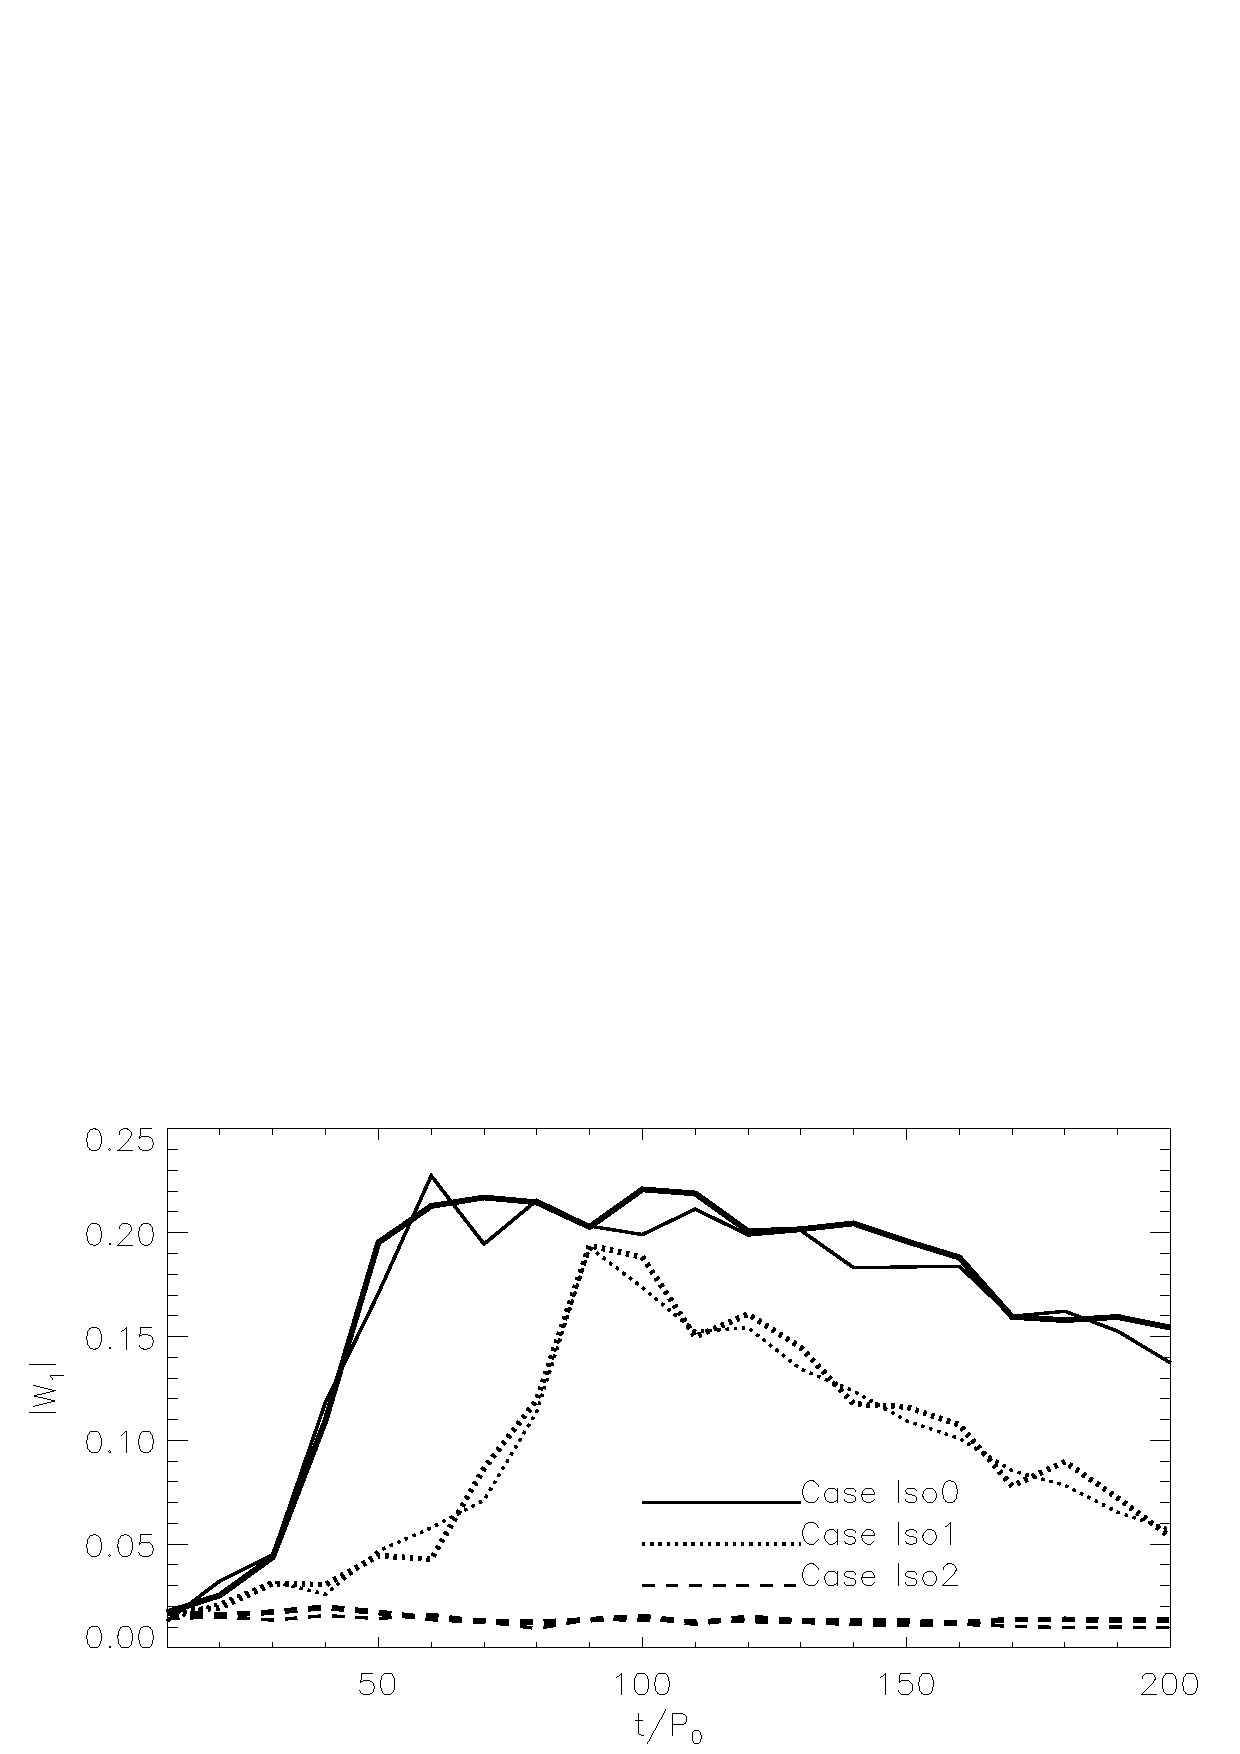
\includegraphics[width=\linewidth]{figures/pdisk_kerz_cases_iso}
  \caption{Same as Fig. \ref{pdisk_kerz_cases_planet} but for strictly
    isothermal Iso0 (solid, no viscous layer so $\hat{\nu}\sim10^{-6}$), Iso1
    (dotted, viscous layer with $\hat{\nu}\sim10^{-5}$) and Iso2
    (dashed, viscous layer with $\hat{\nu}\sim10^{-4}$). The thick (thin) lines indicate
    $W_1$ averaged over $\tan{\psi}\in[0,2]h$
    ($\tan{\psi}\in[2,3]h$).  
    \label{pdisk_kerz_cases_planet_iso}}
\end{figure}
